\documentclass[9pt, aspectratio=169]{beamer}
% \documentclass[10pt]{beamer}
\usepackage[utf8]{inputenc}
\usepackage[T1]{fontenc}
\usepackage[english]{babel}
\usetheme{Frankfurt}

\usepackage[backend=biber, style=authoryear]{biblatex}
\addbibresource{local_references.bib}

%\usepackage{lmodern}
\usepackage{amsfonts,amssymb,amsmath}
\usepackage[english]{babel}
\usetheme{Frankfurt}

\usepackage{csquotes}
\usepackage{setspace}

\usepackage{colortbl}
\usepackage{tabularx}
\renewcommand\tabularxcolumn[1]{m{#1}}

% --- Tickz
\usepackage{physics}
\usepackage{amsmath}
\usepackage{tikz}
\usepackage{mathdots}
\usepackage{yhmath}
\usepackage{cancel}
\usepackage{color}
\usepackage{siunitx}
\usepackage{array}
\usepackage{multirow}
\usepackage{amssymb}
\usepackage{gensymb}
\usepackage{tabularx}
\usepackage{extarrows}
\usepackage{booktabs}
\usetikzlibrary{fadings}
\usetikzlibrary{patterns}
\usetikzlibrary{shadows.blur}
\usetikzlibrary{shapes}

% ---------

\usepackage{booktabs}
\usepackage{setspace}
\usepackage{amssymb}
\usepackage{adjustbox}
\usepackage{pifont}
\usepackage[inkscapeformat=png]{svg}
\usepackage{graphicx}
\usepackage{times}
\setbeamertemplate{caption}[numbered]
% % \setbeamertemplate{bibliography item}{[\theenumiv]}

\setbeamerfont{bibliography item}{size=\tiny}
\setbeamerfont{bibliography entry author}{size=\tiny}
\setbeamerfont{bibliography entry title}{size=\tiny}
\setbeamerfont{bibliography entry location}{size=\tiny}
\setbeamerfont{bibliography entry note}{size=\tiny}

\setbeamerfont{frametitle}{size=\large}

\usepackage{caption}
\usepackage{float}
\usepackage{xcolor}
\usepackage{listings}
\usepackage{animate}

\definecolor{codegreen}{rgb}{0,0.6,0}
\definecolor{codegray}{rgb}{0.5,0.5,0.5}
\definecolor{codepurple}{rgb}{0.58,0,0.82}
\definecolor{backcolour}{rgb}{0.95,0.95,0.92}
 
\lstdefinestyle{mystyle}{
    backgroundcolor=\color{backcolour},   
    commentstyle=\color{codegreen},
    keywordstyle=\color{magenta},
    numberstyle=\tiny\color{codegray},
    stringstyle=\color{codepurple},
    basicstyle=\footnotesize,
    breakatwhitespace=false,         
    breaklines=true,                 
    captionpos=b,                    
    keepspaces=true,                 
    numbers=left,                    
    numbersep=5pt,                  
    showspaces=false,                
    showstringspaces=false,
    showtabs=false,                  
    tabsize=2
}
 
\lstset{style=mystyle}

\usepackage{ragged2e}
\setbeamercolor{section in foot}{fg=white,bg=darkorange}
\setbeamercolor{subsection in foot}{fg=white,bg=darkorange}
\setbeamercolor{frametitle}{fg=white, bg=darkorange}
\setbeamercolor{title}{fg=white, bg=darkorange}
\setbeamercolor{frame}{bg=darkorange}
\setbeamercolor{block title}{bg=darkorange,fg=white}

\setbeamercolor{item}{fg=darkorange}

% \definecolor{darkorange}{rgb}{0.81, 0.52, 0.05}
\definecolor{darkorange}{rgb}{1,0.5,0}
\definecolor{darkorange2}{rgb}{1, 0.64, 0.2}
\definecolor{honeydew}{rgb}{1, 0.85, 0.45}


\newenvironment{variableblock}[3]{%
  \setbeamercolor{block body}{#2}
  \setbeamercolor{block title}{#3}
  \begin{block}{#1}}{\end{block}}

\newenvironment{prosblock}[1]{%
  % \setbeamercolor{block body}{bg=blue,fg=white}
  \setbeamercolor{block title}{bg=blue,fg=white}
  \begin{block}{#1}}{\end{block}}

\newenvironment{consblock}[1]{%
  % \setbeamercolor{block body}{bg=red,fg=white}
  \setbeamercolor{block title}{bg=red,fg=white}
  \begin{block}{#1}}{\end{block}}

\newcommand{\cmark}{\ding{51}}%
\newcommand{\xmark}{\ding{55}}%

\renewcommand{\arraystretch}{1.5}

% Please add the following required packages to your document preamble:
\usepackage{booktabs}
\usepackage{multirow}
\usepackage{colortbl}
% Beamer presentation requires \usepackage{colortbl} instead of \usepackage[table,xcdraw]{xcolor}

\usepackage{tabularray}\UseTblrLibrary{varwidth}
\usepackage{xcolor}
\def\BibTeX{{\rm B\kern-.05em{\sc i\kern-.025em b}\kern-.08em
    T\kern-.1667em\lower.7ex\hbox{E}\kern-.125emX}}
% \usepackage{cite}
\usepackage{amsmath}
\newcommand{\probP}{\text{I\kern-0.15em P}}
\usepackage{etoolbox}
\patchcmd{\thebibliography}{\section*{\refname}}{}{}{}

\setlength\tabcolsep{0.5pt}

\renewcommand{\arraystretch}{0.9}
\setlength{\tabcolsep}{2pt}

\usepackage{pgffor}

\setbeamerfont{bibliography item}{size=\tiny}
\setbeamerfont{bibliography entry author}{size=\tiny}
\setbeamerfont{bibliography entry title}{size=\tiny}
\setbeamerfont{bibliography entry location}{size=\tiny}
\setbeamerfont{bibliography entry note}{size=\tiny}

\setbeamerfont{bibliography entry author}{shape=\upshape,series=\mdseries,size=\footnotesize}
\setbeamerfont{bibliography entry title}{shape=\slshape,series=\mdseries,size=\footnotesize}
\setbeamerfont{bibliography entry journal}{shape=\upshape,series=\mdseries,size=\footnotesize}
\setbeamerfont{bibliography entry note}{shape=\upshape,series=\mdseries,size=\footnotesize}

\renewcommand*{\bibfont}{\scriptsize}

\newenvironment<>{varblock}[2][.9\textwidth]{%
  \setlength{\textwidth}{#1}
  \begin{actionenv}#3%
    \def\insertblocktitle{#2}%
    \par%
    \usebeamertemplate{block begin}}
  {\par%
    \usebeamertemplate{block end}%
  \end{actionenv}}

% \setbeamertemplate{footline}[frame number]

\setbeamertemplate{footline}{
  \leavevmode%
  \hfill
  \usebeamercolor[fg]{page number in head/foot}%
  \scriptsize%
  \ifnum\value{framenumber}>22%
    Appendix \number\numexpr\value{framenumber}-22\relax/26%
  \else%
    \ifnum\value{framenumber}>19%
      %
    \else
      \number\numexpr\value{framenumber}\relax/19%
    \fi

  \fi%
  \hspace{1em}
}


\begin{document}

\author{\textbf{Julien Soulé}, Jean-Paul Jamont, Michel Occello, Paul Théron, Louis-Marie Traonouez}

\title{\textbf{Towards a Multi-Agent Simulation of Cyber-attackers and Cyber-defenders Battles}}

\subtitle{SMC 2023 Presentation}

% \logo{
\includegraphics[scale=0.01]{figures/grenoble-inp_logo.png}}

\institute{\footnotesize \textit{University Grenoble Alpes, Grenoble
INP, LCIS, 26000, Valence, France \\
julien.soule@lcis.grenoble-inp.fr}}

\date{\textit{\footnotesize \today}}

%\subject{}
\setbeamercovered{transparent}
%\setbeamertemplate{navigation symbols}{}
\begin{frame}[plain]
	\maketitle\vspace{-0.8cm}
	\begin{figure}[ht!]
		\centering
            
\includegraphics[height=0.8cm]{figures/la-ruche_logo.png}
            \hspace{0.8cm}
            
\includegraphics[height=0.8cm]{figures/lcis_logo.png}
            \hspace{0.8cm}
		
\includegraphics[height=0.8cm]{figures/grenoble-inp_logo.png}
            \hspace{0.8cm}
            
\includegraphics[height=0.8cm]{figures/uga_logo.jpg}
	\end{figure}
\end{frame}

% \begin{frame}{Content}
%   \tableofcontents
% \end{frame}

\addtocounter{framenumber}{-1}

\section{Introduction}

\begin{frame}{Un sens émergent de l'organisation dans le MARL ?}

  \begin{columns}[T]

    \hspace{-0.5cm}
    \begin{column}{0.3\textwidth}

      \vspace{1cm}
      \begin{itemize}
        \item Même sans instructions explicites, certains motifs comportementaux distincts émergent.
        \item Dans certaines configurations, ces comportements ressemblent à des \textbf{rôles} (et \textbf{objectifs}) définis par des humains.
        \item Mais dans autres cas, coordination reste ambiguë.
      \end{itemize}

    \end{column}

    \begin{column}{0.8\textwidth}

      \begin{columns}[T]
        \begin{column}{0.48\textwidth}
          \centering
          \animategraphics[autoplay,loop,width=0.8\linewidth]{8}{figures/overcooked_asymmetric_advantage/frame}{0}{33} \\
          \small{\textbf{Avantage Asymétrique}}\\
          \vspace{0.3em}
          \animategraphics[autoplay,loop,width=0.7\linewidth]{8}{figures/overcooked_coordination_ring/frame}{0}{33} \\
          \small{\textbf{Anneau de Coordination}}
        \end{column}
        \begin{column}{0.48\textwidth}
          \centering
          \animategraphics[autoplay,loop,width=0.75\linewidth]{8}{figures/overcooked_counter_circuit/frame}{0}{33} \\
          \small{\textbf{Circuit de Comptoir}}\\
          \vspace{0.3em}
          \animategraphics[autoplay,loop,width=0.7\linewidth]{8}{figures/overcooked_forced_coordination/frame}{0}{33} \\
          \small{\textbf{Coordination Forcée}}
        \end{column}
      \end{columns}

    \end{column}

  \end{columns}

  \hspace{-1cm}
  \vspace{-0.5cm}
  {\tiny \textit{Overcooked-AI~\autocite{overcookedai}}}

\end{frame}

\begin{frame}{De motifs émergents à l'adéquation organisationnelle}

  \begin{columns}[c]
    % COLONNE GAUCHE : comportement appris
    \begin{column}{0.48\textwidth}
      \centering
      \animategraphics[autoplay,loop,width=0.95\linewidth]{8}{figures/overcooked_asymmetric_advantage/frame}{0}{33} \\
      \small\textbf{Comportement Appris (après MARL)}
    \end{column}

    % COLONNE DROITE : comportement idéal défini par l'humain
    \begin{column}{0.48\textwidth}
      \centering
      \animategraphics[autoplay,loop,width=0.95\linewidth]{8}{figures/clean_overcooked_asymmetric_advantage/frame}{0}{33} \\
      \small\textbf{Organisation Régulière (conçue par des humains)}
    \end{column}
  \end{columns}

  \vspace{1em}

  \begin{itemize}
    \item Agents entraînés peuvent manifester régularités comportementales proches d'une \textbf{organisation implicite} comprenant spécifications \textquote{débruitées}:
          \begin{itemize}
            \item \textbf{Structurelles} — rôles réguliers
            \item \textbf{Fonctionnelles} — objectifs réguliers
          \end{itemize}
  \end{itemize}

  \begin{block}{\textbf{Adéquation organisationnelle} : un concept pratique proposé comme\dots}
    La \textquote{distance} entre comportements des agents entraînés et ceux de organisation implicite.
  \end{block}

\end{frame}

\begin{frame}{Jusqu'où peut-on pousser le concept d'adéquation organisationnelle ?}

  \begin{block}{\textbf{Voir les agents MARL à travers le prisme organisationnel ?}}

    Deux questions de recherche centrales :

    \begin{enumerate}
      \item \textbf{Comment peut-on évaluer l'adéquation organisationnelle ?} \\
            Mesurer dans quelle mesure les comportements des agents correspondent à une organisation fonctionnelle et structurée ?

            \vspace{0.8em}
      \item \textbf{Comment peut-on contrôler l'adéquation organisationnelle ?} \\
            Guider l'entraînement des agents pour qu'ils s'alignent avec des rôles et objectifs prédéfinis ?
    \end{enumerate}

  \end{block}

\end{frame}

\section{Travaux connexes \& Contribution}

\begin{frame}{Travaux connexes \& Contribution}{Évaluation/Contrôle de l'adéquation organisationnelle ?}

  \begin{columns}
    \vspace{-0.7cm}
    \begin{column}{0.35\textwidth}
      \centering
      \begin{block}{Limitations}
        \begin{footnotesize}
          \begin{itemize}
            \item Aucun équivalent direct du concept d'adéquation organisationnelle.
            \item Aucun moyen systématique de quantifier dans quelle mesure les comportements appris s'alignent avec une organisation implicite ou donnée.
            \item Aucun cadre général pour contrôler ou guider les agents de manière organisationnelle.
          \end{itemize}
        \end{footnotesize}
      \end{block}
      \begin{exampleblock}{Contribution}
        Modèle organisationnel + MARL ? \\ \ \ \ \ $\rightarrow$ \textbf{MOISE+MARL}
      \end{exampleblock}
    \end{column}
    \hspace{0.1cm}
    \begin{column}{0.7\textwidth}
      \centering
      \begin{footnotesize}
        \textquote{Contrôle de l'adéquation organisationnelle} ?
        \begin{itemize}
          \item Wilson et al.~\autocite{wilson2008learning} : Transfert de rôles entre environnements dans des MDP multi-agents, mais manque d'abstraction.
          \item Berenji et Vengerov~\autocite{berenji2000learning} : Coordination et inférence de rôles dans des UAVs — spécifique à une tâche, non généralisable.
          \item Yusuf et Baber~\autocite{yusuf2020inferential} : Inférence bayésienne pour la coordination de tâches — sans métriques d'alignement organisationnel.
          \item Serrino et al.~\autocite{serrino2019finding} : Inférence de rôles sociaux à partir d'interactions — limité à des rôles opérationnels à court terme.
        \end{itemize}

        \vspace{0.5cm}

        \textquote{Évaluation de l'adéquation organisationnelle} ?
        \begin{itemize}
          \item CPO~\autocite{achiam2017cpo} : Contraintes de sûreté pour régulariser l'apprentissage — pas d'extension aux contraintes organisationnelles.
          \item Ray et al.~\autocite{ray2019benchmarking} : Shaping de récompense lagrangienne — pas de contraintes sur des espaces d'action dynamiques.
          \item \textit{Safe exploration}~\autocite{garcia2015comprehensive,alshiekh2018safe} : Vise à éviter les états dangereux — sans respect des rôles.
          \item HRL~\autocite{ghavamzadeh2006hrl} : Décomposition de tâches alignée avec des hiérarchies — mais imposée de manière interne.
        \end{itemize}
      \end{footnotesize}
    \end{column}
  \end{columns}

\end{frame}

\section{Cadre MOISE+MARL}

\begin{frame}{Cadre MOISE+MARL}{Le cadre $\mathcal{M}OISE^+$ (1/2)}

  \begin{figure}
    \centering
    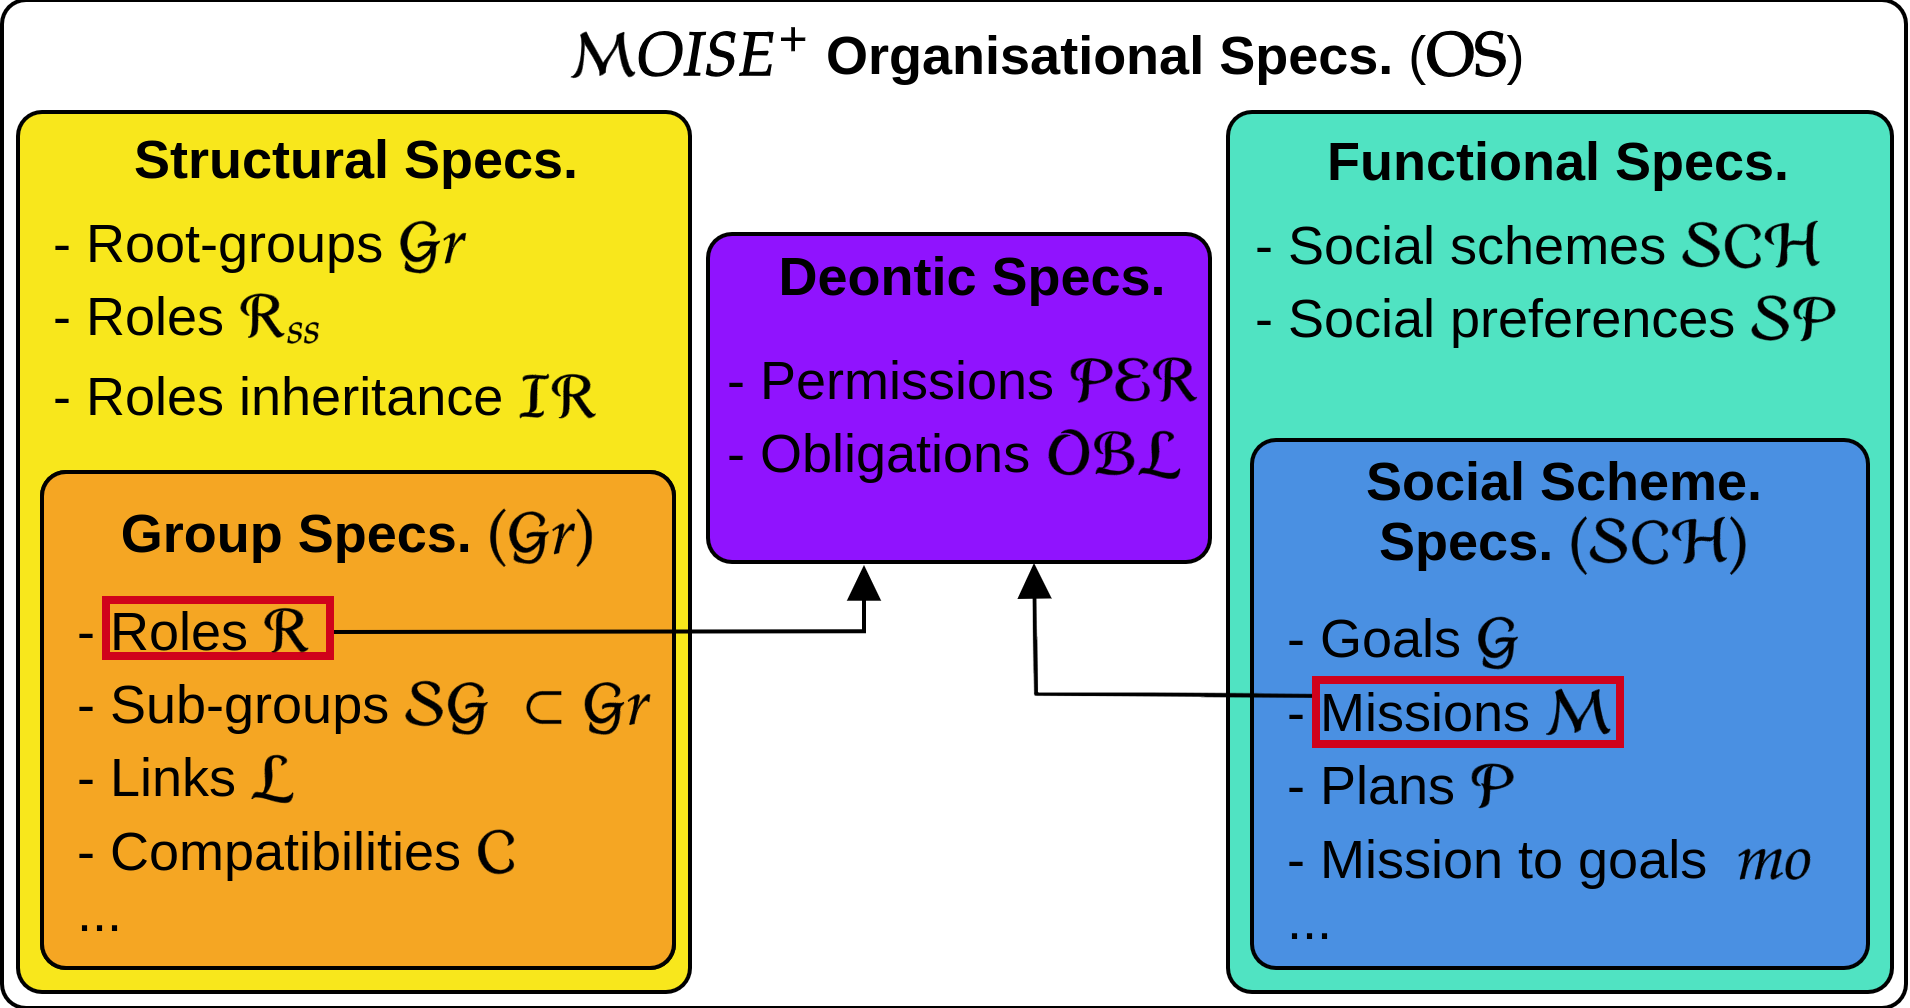
\includegraphics[width=0.75\linewidth]{figures/moise_model.png}
  \end{figure}

  \begin{spacing}{0.25}
    {\tiny Hübner, J. F., Sichman, J. S., and Boissier, O. (2002).
      Un modèle pour la spécification structurelle, fonctionnelle et déontique
      des organisations dans les systèmes multi-agents.
      In Bittencourt, G. et Ramalho, G. L., éditeurs, Actes du 16ème Symposium Brésilien sur l'Intelligence Artificielle (SBIA'02), volume 2507 de LNAI, pages 118–128, Berlin. Springer.}
  \end{spacing}

\end{frame}

\begin{frame}{Le cadre MOISE+MARL}{Modèle markovien}

  \begin{columns}

    \hspace{-2ex}

    \begin{column}{0.4\textwidth}

      \begin{figure}
        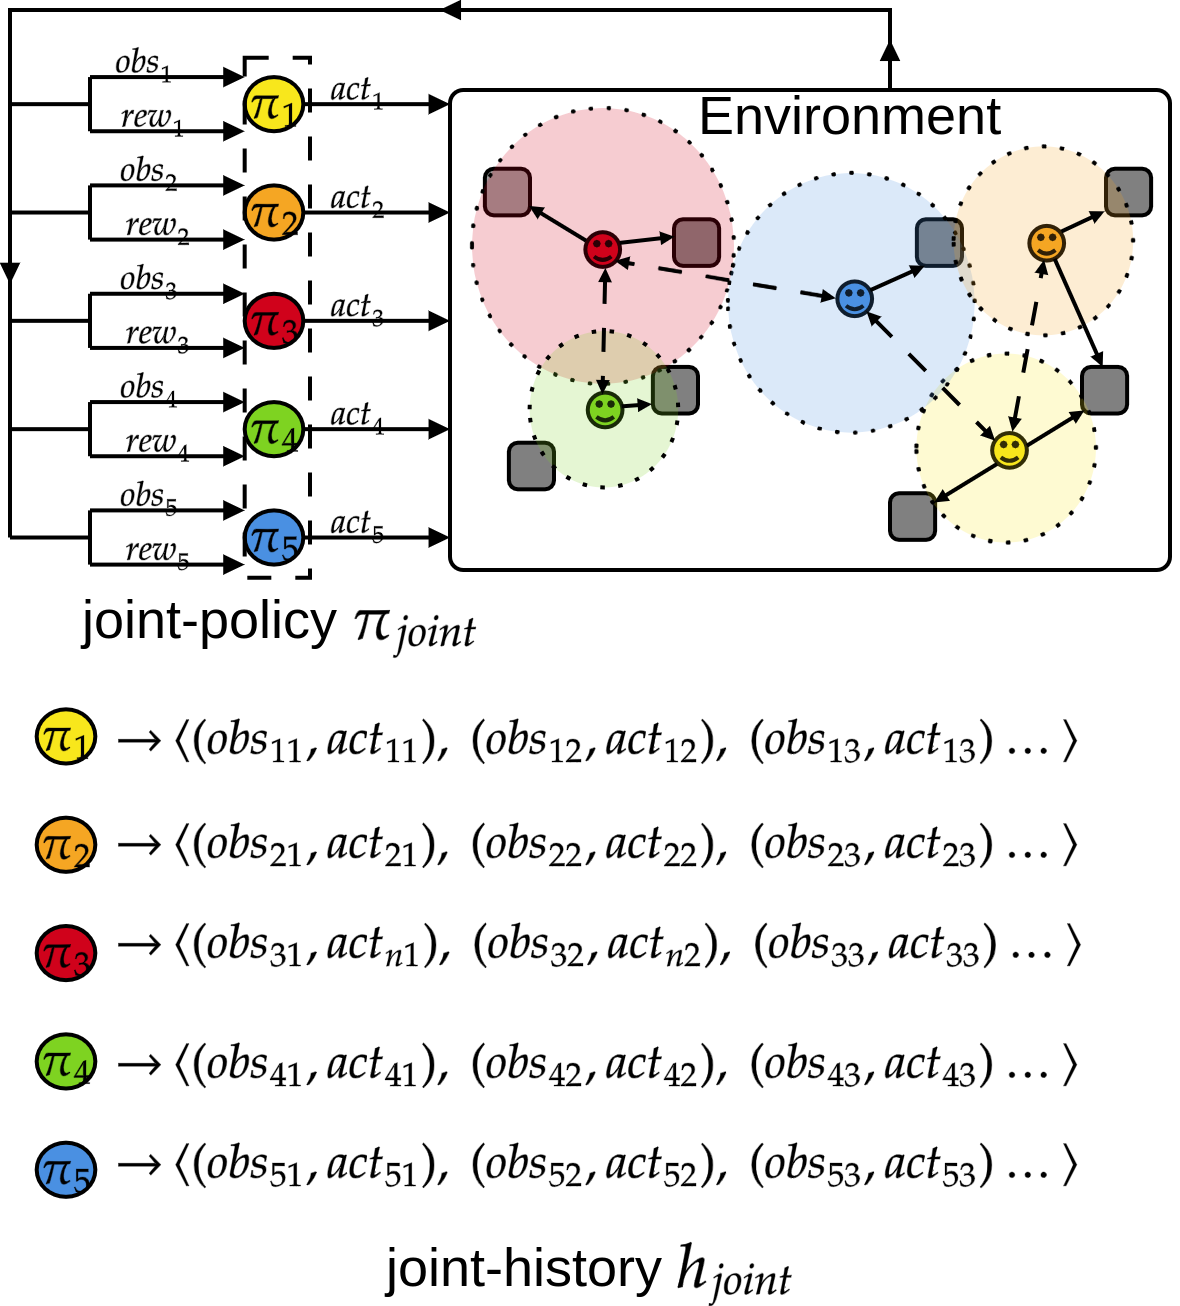
\includegraphics[width=\linewidth]{figures/marl_basics.png}
      \end{figure}

    \end{column}

    \begin{column}{0.7\textwidth}
      \vspace{-2ex}

      \begin{center}
        \begin{minipage}{0.95\linewidth}
          \centering
          \begin{block}{Modèles markoviens pour le MARL : Dec-POMDP}
            {\small
              Processus Décisionnel de Markov Partiellement Observable et Décentralisé (Dec-POMDP)~\autocite{Oliehoek2016}
              \begin{itemize}
                \item considère plusieurs agents dans une approche MAS similaire ;
                \item processus stochastiques pour modéliser l'incertitude des changements environnementaux, y compris les observations ;
                \item fonction de récompense commune aux agents, favorisant l'apprentissage d'actions collaboratives~\autocite{Beynier2013}
              \end{itemize}
            }

            { \scriptsize

              $(S,\{A_i\},T,R,\{\Omega_i\},O,\gamma)$ , où
              \begin{itemize}
                \item $S = \{s_1, ..s_{|S|}\}$ : ensemble des états possibles ;
                \item $A_{i} = \{a_{1}^{i},..,a_{|A_{i}|}^{i}\}$ : ensemble des actions possibles pour l'agent $i$ ;
                \item $T$ tel que $T(s,a,s') = \probP{(s'|s,a)}$ : probabilités de transition conditionnelles ;
                \item $R: S \times A \times S \rightarrow \mathbb{R}$ : fonction de récompense ;
                \item $\Omega_{i} = \{o_{1}^{i},..,o_{|\Omega_{i}|}^{i}\}$ : ensemble des observations pour l'agent $ag_i$ ;
                \item $O$ tel que $O(s',a,o) = \probP{(o|s',a)}$ : probabilités conditionnelles d'observation ;
                \item $\gamma \in [0,1]$ : facteur d'actualisation.
              \end{itemize}

            }

          \end{block}

        \end{minipage}
      \end{center}

    \end{column}

  \end{columns}

\end{frame}

\begin{frame}{Le cadre MOISE+MARL}{Approche}

  \begin{columns}[c]

    \begin{column}{0.5\textwidth}

      \begin{itemize}
        \item Combiner Dec-POMDP avec le modèle organisationnel $\mathcal{M}OISE^+$.
        \item Les agents se voient attribuer des rôles et des missions.
        \item Utiliser des guides de contraintes pour ajuster :
              \begin{itemize}
                \item \textbf{Actions} via \textbf{Guides d'Actions par Rôle} (RAG)
                \item \textbf{Récompenses} via \textbf{Guides de Récompense par Rôle} (RRG) et \textbf{Guides de Récompense par Objectif} (GRG)
              \end{itemize}
      \end{itemize}

      \noindent
      \hspace{0.5cm}
      \begin{minipage}{\linewidth}
        \begin{varblock}[5.5cm]{Implémentation des \textbf{rôles} et \textbf{objectifs} $\sim$ \textbf{Guides de Contrainte}}

          \begin{itemize}
            \item $rag: H \times \Omega \rightarrow \mathcal{P}(A \times \mathbb{R})$
            \item $rrg: H \times \Omega \times A \to \mathbb{R}$
            \item $grg: H \rightarrow \mathbb{R}$
          \end{itemize}

        \end{varblock}
      \end{minipage}

    \end{column}

    \hspace{-0.2cm}

    \begin{column}{0.6\textwidth}
      \begin{figure}
        \centering
        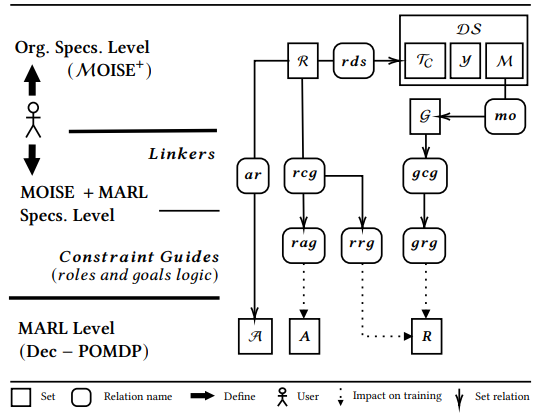
\includegraphics[width=1.\linewidth]{figures/mm_simple_representation.png}
      \end{figure}
    \end{column}
  \end{columns}
\end{frame}

\begin{frame}{Le cadre MOISE+MARL}{Approche}

  \begin{figure}
    \centering
    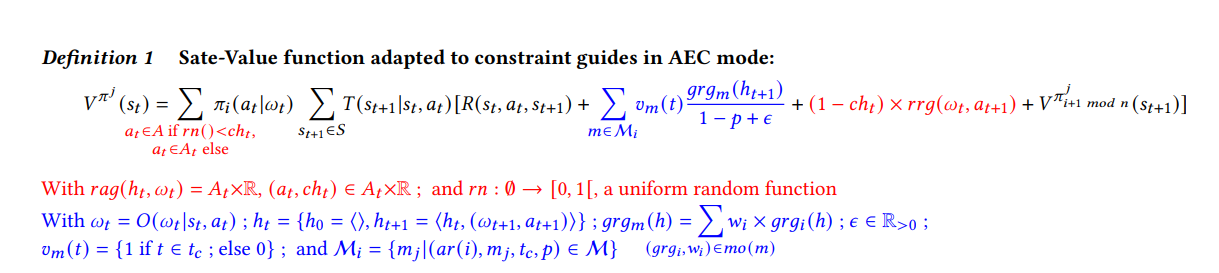
\includegraphics[width=1.07\linewidth]{figures/modified_state_value_function.png}

    \

    \phantom{X}\\

    \begin{tikzpicture}
      \fill[black] (0,0) rectangle +(0.3,0.3);
      \node[right=0.4cm] at (0.3,0.15) {\small \textbf{MARL standard (fonction de valeur d'état originale)}};
      \fill[red] (0,-0.8) rectangle +(0.3,0.3);
      \node[right=0.4cm] at (0.3,-0.65) {\small \textbf{Guidage par rôle (RAG, RRG)}};
      \fill[blue] (0,-1.6) rectangle +(0.3,0.3);
      \node[right=0.4cm] at (0.3,-1.45) {\small \textbf{Guidage par objectif (GRG)}};
    \end{tikzpicture}

  \end{figure}

  \begin{tikzpicture}[remember picture, overlay]

    \node[anchor=north west, draw=red, fill=red, text=white, rounded corners=1pt, inner sep=2pt]
    at ([xshift=1.3cm,yshift=-3.69cm]current page.north west) {\small \textit{RAG}};

    \node[anchor=north west, draw=red, fill=red, text=white, rounded corners=1pt, inner sep=2pt]
    at ([xshift=11.5cm,yshift=-3.69cm]current page.north west) {\small \textit{RRG}};

    \node[anchor=north west, draw=blue, fill=blue, text=white, rounded corners=1pt, inner sep=2pt]
    at ([xshift=9.1cm,yshift=-3.69cm]current page.north west) {\small \textit{GRG}};

  \end{tikzpicture}

\end{frame}

\begin{frame}{Le cadre MOISE+MARL}{Défis dans la définition des guides de contrainte (RAG, RRG, GRG)}

    \textbf{Problème :} Définir les guides de contrainte dans le MARL est un défi en pratique.

    \begin{itemize}
        \item Une spécification complète \textquote{par extension} est peu praticable :
              \begin{itemize}
                  \item Énumérer tous les cas possibles d’observation ou d’historique est intraitable.
                  \item Maintenir et mettre à jour de telles règles ne passe pas à l’échelle.
              \end{itemize}

        \item \textbf{Nous proposons deux stratégies intensionnelles pour définir les guides de contrainte :}
              \begin{enumerate}
                  \item \textbf{Scripts logiques personnalisés :} L’utilisateur définit des fonctions Python (par rôle/objectif) qui prennent en entrée une trajectoire et une observation, et retournent :
                        \begin{itemize}
                            \item RAG : actions autorisées avec des poids de difficulté
                            \item RRG : pénalités ou bonus de récompense pour certaines actions
                            \item GRG : shaping de récompense basé sur des caractéristiques de trajectoire
                        \end{itemize}
                  \item \textbf{\textit{Trajectory-based Pattern} (TPs) :} Patrons déclaratifs compacts inspirés du traitement du langage naturel, utilisés pour représenter des comportements.
              \end{enumerate}
    \end{itemize}

\end{frame}

%==================================================

\begin{frame}{Le cadre MOISE+MARL}{Solution 1 : Guides de contrainte via scripts personnalisés}

    \textbf{Principe :} Définir une fonction par rôle/objectif qui analyse la trajectoire et l'observation actuelle.

    \vspace{0.5em}
    \textbf{Exemple (Overcooked-AI) :}

    \begin{itemize}
        \item \textbf{Rôle :} Cuisinier principal
        \item \textbf{Observation :} L’agent tient une assiette, une casserole est prête, pas de mur devant
        \item \textbf{Trajectoire :} L’agent a précédemment pris un oignon, puis l’a découpé
    \end{itemize}

    \textbf{Sortie du script :}

    \begin{itemize}
        \item \textbf{RAG :} \{`interact' $\rightarrow$ 1.0, `nothing' $\rightarrow$ 0.2\}
        \item \textbf{RRG :} Bonus de +2 si `interact` est utilisé à proximité d’une casserole prête
        \item \textbf{GRG :} +1 si la trajectoire se termine par une livraison de soupe
    \end{itemize}

    \textbf{Avantage :} La logique personnalisée peut prendre en compte la disposition spatiale, les étapes précédentes, l’objet tenu, etc.

\end{frame}

%==================================================

\begin{frame}{Le cadre MOISE+MARL}{Solution 2 : Guides de contrainte via \textit{Trajectory-based Pattern} (TPs)}

    \textbf{Principe :} Définir des \textit{Trajectory-based Pattern} réutilisables et lisibles par un humain pour correspondre au comportement d’un agent.

    \vspace{0.5em}
    \textbf{Format :} TP = transitions décrites comme \textbf{\textit{[obs, act | sub\_TP]($n_{min}$, $n_{max}$)}}

    \textbf{Exemple (Overcooked-AI) :}

    \begin{itemize}
        \item \textbf{Patron :} \\ \textit{[`see\_onion`, `interact`, [\#any](*), `see\_chopped`, `interact`, [\#any](*), `see\_pot`, `interact`](1,1)}
        \item \textbf{Correspondance TP :} L’agent a rempli une casserole avec un oignon découpé
        \item \textbf{Observation actuelle :} \texttt{see\_ready\_pot}
    \end{itemize}

    \textbf{Alors :}
    \begin{itemize}
        \item \textbf{RAG :} Autoriser uniquement l’action `interact`
        \item \textbf{RRG :} Bonus de +3 pour `interact` maintenant
        \item \textbf{GRG :} Encourager à se diriger vers la zone de livraison ensuite
    \end{itemize}

    \textbf{Avantages :}
    \begin{itemize}
        \item Plus facile de définir des patrons symboliques dans divers environnements
        \item Codage compact de comportements temporellement étendus
        \item Les TPs peuvent être réutilisés entre agents et rôles
    \end{itemize}

\end{frame}

\begin{frame}{Le cadre MOISE+MARL}{Présentation de la méthode TEMM}

  \textbf{Évaluation basée sur les trajectoires dans MOISE+MARL (TEMM)}
  \begin{itemize}
    \item \textbf{Objectif} : Fournir une interprétation organisationnelle du comportement des agents entraînés.
  \end{itemize}

  \vspace{1em}
  \textbf{Hypothèses sous-jacentes :}
  \begin{itemize}
    \item \textbf{Rôles} $\sim$ motifs fréquents de transitions \emph{(observation, action)} dans les trajectoires des agents.
    \item \textbf{Objectifs} $\sim$ observations reçues fréquemment dans les trajectoires.
  \end{itemize}

  \begin{center}
    \begin{columns}[c]

      \begin{column}{0.4\textwidth}
        \centering
        


\tikzset{every picture/.style={line width=0.75pt}} %set default line width to 0.75pt        

\begin{tikzpicture}[x=0.75pt,y=0.75pt,yscale=-1,xscale=1]
%uncomment if require: \path (0,1974); %set diagram left start at 0, and has height of 1974

%Shape: Rectangle [id:dp21508130618742183] 
\draw  [fill={rgb, 255:red, 255; green, 255; blue, 255 }  ,fill opacity=1 ] (27.9,1694.11) -- (180,1694.11) -- (180,1780) -- (27.9,1780) -- cycle ;
%Straight Lines [id:da4715774117452397] 
\draw [color={rgb, 255:red, 208; green, 2; blue, 27 }  ,draw opacity=1 ]   (146.57,1706.84) -- (128.18,1713.49) -- (91.16,1728.41) -- (112.58,1740.12) -- (97.43,1737.36) -- (90.48,1739.01) -- (90.48,1748.77) -- (85.95,1752.07) -- (85.12,1752.67) -- (82.55,1750.8) -- (74.41,1744.86) -- (58.34,1744.86) -- (60.9,1746.73) -- (52.99,1748.77) -- (55.75,1752.79) -- (42.28,1764.38) ;
\draw [shift={(149.39,1705.82)}, rotate = 160.12] [fill={rgb, 255:red, 208; green, 2; blue, 27 }  ,fill opacity=1 ][line width=0.08]  [draw opacity=0] (3.57,-1.72) -- (0,0) -- (3.57,1.72) -- cycle    ;
%Straight Lines [id:da12621479480258224] 
\draw [color={rgb, 255:red, 80; green, 227; blue, 194 }  ,draw opacity=1 ]   (147.37,1704.13) -- (138.68,1713.63) -- (117.26,1713.63) -- (117.26,1721.44) -- (90.48,1729.25) -- (95.83,1733.15) -- (101.19,1740.96) -- (85.12,1737.06) -- (90.48,1744.86) -- (85.12,1744.86) -- (90.48,1752.67) -- (79.77,1752.67) -- (71.84,1744.94) -- (69.05,1750.72) -- (47.63,1739.01) -- (63.7,1752.67) -- (47.63,1744.86) -- (52.99,1752.67) -- (47.63,1768.29) ;
\draw [shift={(149.39,1701.92)}, rotate = 132.45] [fill={rgb, 255:red, 80; green, 227; blue, 194 }  ,fill opacity=1 ][line width=0.08]  [draw opacity=0] (3.57,-1.72) -- (0,0) -- (3.57,1.72) -- cycle    ;
%Straight Lines [id:da7064890769152855] 
\draw [color={rgb, 255:red, 248; green, 231; blue, 28 }  ,draw opacity=1 ]   (157.13,1710.14) -- (130.73,1713.75) -- (127.97,1717.54) -- (109.3,1721.56) -- (95.83,1729.25) -- (97.43,1737.36) -- (93.24,1741.08) -- (85.12,1733.15) -- (95.83,1748.77) -- (95.83,1752.67) -- (85.12,1752.67) -- (63.89,1745.06) -- (61.1,1750.84) -- (45.04,1752.79) -- (39.68,1768.41) ;
\draw [shift={(160.1,1709.73)}, rotate = 172.2] [fill={rgb, 255:red, 248; green, 231; blue, 28 }  ,fill opacity=1 ][line width=0.08]  [draw opacity=0] (3.57,-1.72) -- (0,0) -- (3.57,1.72) -- cycle    ;
%Straight Lines [id:da7638374972620724] 
\draw [color={rgb, 255:red, 144; green, 19; blue, 254 }  ,draw opacity=1 ]   (164.12,1713.39) -- (169.74,1714.41) -- (165.46,1709.73) -- (161.17,1706.61) -- (168.76,1709.73) -- (174.03,1714.41) -- (165.46,1719.1) -- (170.81,1725.34) -- (165.46,1733.15) -- (170.81,1737.06) -- (165.46,1748.77) -- (165.46,1764.38) -- (149.39,1760.48) -- (138.68,1760.48) -- (132.88,1759.07) -- (129.82,1758.33) -- (125.47,1757.27) -- (122.61,1756.58) -- (111.86,1755.71) -- (103.33,1755.01) -- (99.13,1754.25) -- (90.48,1752.67) -- (79.77,1752.67) -- (74.41,1756.58) -- (63.7,1760.48) -- (63.7,1768.29) ;
\draw [shift={(161.17,1712.85)}, rotate = 10.33] [fill={rgb, 255:red, 144; green, 19; blue, 254 }  ,fill opacity=1 ][line width=0.08]  [draw opacity=0] (3.57,-1.72) -- (0,0) -- (3.57,1.72) -- cycle    ;
%Straight Lines [id:da2586635599751653] 
\draw [color={rgb, 255:red, 65; green, 117; blue, 5 }  ,draw opacity=1 ]   (163.05,1714.17) -- (168.67,1715.19) -- (164.39,1710.51) -- (160.1,1707.39) -- (167.69,1710.51) -- (172.95,1715.19) -- (165.46,1723.78) -- (169.74,1726.13) -- (167.6,1737.84) -- (154.75,1733.15) -- (165.46,1739.4) -- (178.31,1751.89) -- (161.17,1742.52) -- (164.39,1749.55) -- (167.6,1761.26) -- (156.89,1764.38) -- (139.75,1758.14) -- (126.9,1758.14) -- (120.47,1758.14) -- (114.04,1756.58) -- (111.9,1759.7) -- (107.62,1756.58) -- (109.76,1761.26) -- (98.06,1755.03) -- (89.41,1753.45) -- (78.69,1753.45) -- (73.34,1757.36) -- (62.63,1761.26) -- (62.63,1769.07) ;
\draw [shift={(160.1,1713.63)}, rotate = 10.33] [fill={rgb, 255:red, 65; green, 117; blue, 5 }  ,fill opacity=1 ][line width=0.08]  [draw opacity=0] (3.57,-1.72) -- (0,0) -- (3.57,1.72) -- cycle    ;
%Shape: Polygon Curved [id:ds11407168049221061] 
\draw  [color={rgb, 255:red, 74; green, 144; blue, 226 }  ,draw opacity=1 ][fill={rgb, 255:red, 74; green, 144; blue, 226 }  ,fill opacity=0.5 ] (31.11,1764.38) .. controls (34.28,1759.39) and (40.53,1757.99) .. (46.46,1758.18) .. controls (50.95,1758.33) and (55.26,1759.39) .. (57.89,1760.48) .. controls (64,1763.02) and (69.46,1762.63) .. (68.6,1768.29) .. controls (67.74,1773.95) and (60.78,1773.17) .. (52.53,1772.19) .. controls (44.29,1771.22) and (25.54,1773.17) .. (31.11,1764.38) -- cycle ;
%Shape: Polygon Curved [id:ds9280877944894264] 
\draw  [color={rgb, 255:red, 208; green, 2; blue, 27 }  ,draw opacity=1 ][fill={rgb, 255:red, 208; green, 2; blue, 27 }  ,fill opacity=0.5 ] (143.58,1705.82) .. controls (149.15,1697.04) and (151.91,1697.59) .. (148.94,1701.92) .. controls (145.97,1706.25) and (158.58,1699.87) .. (157.72,1705.53) .. controls (156.86,1711.19) and (173.25,1714.61) .. (165,1713.63) .. controls (156.76,1712.66) and (138.01,1714.61) .. (143.58,1705.82) -- cycle ;


% Text Node
\draw (109.47,1704.35) node  [font=\tiny,color={rgb, 255:red, 202; green, 52; blue, 69 }  ,opacity=1 ] [align=left] {$\displaystyle g_{*} =\Omega _{goal}$};
% Text Node
\draw (77.33,1773.35) node  [font=\tiny,color={rgb, 255:red, 74; green, 144; blue, 226 }  ,opacity=1 ] [align=left] {$\displaystyle \Omega _{init}$};
% Text Node
\draw (37,1704) node  [font=\scriptsize] [align=left] {$\displaystyle \Omega $};
% Text Node
\draw (96.51,1791) node   [align=left] {{\tiny \textit{An abstract visualization of}}};
\draw (96.51,1800) node   [align=left] {{\tiny \textit{observations in trajectories}}};

\end{tikzpicture}
      \end{column}

      \begin{column}{0.1\textwidth}
      \end{column}

      \begin{column}{0.4\textwidth}
        \centering
        


\tikzset{every picture/.style={line width=0.75pt}} %set default line width to 0.75pt        

\begin{tikzpicture}[x=0.75pt,y=0.75pt,yscale=-1,xscale=1]
%uncomment if require: \path (0,1974); %set diagram left start at 0, and has height of 1974

%Shape: Rectangle [id:dp10581972605309897] 
\draw  [fill={rgb, 255:red, 255; green, 255; blue, 255 }  ,fill opacity=1 ] (189.9,1694) -- (342,1694) -- (342,1779.89) -- (189.9,1779.89) -- cycle ;
%Straight Lines [id:da15954508078344698] 
\draw [color={rgb, 255:red, 208; green, 2; blue, 27 }  ,draw opacity=1 ]   (308.57,1706.73) -- (290.18,1713.38) -- (253.16,1728.29) -- (292,1737.89) -- (274,1745.89) -- (262,1749.89) -- (252.48,1748.66) -- (246,1737.89) -- (240,1737.89) -- (236,1739.89) -- (236.41,1744.75) -- (220.34,1744.75) -- (222.9,1746.61) -- (214.99,1748.66) -- (217.75,1752.68) -- (204.28,1764.27) ;
\draw [shift={(311.39,1705.71)}, rotate = 160.12] [fill={rgb, 255:red, 208; green, 2; blue, 27 }  ,fill opacity=1 ][line width=0.08]  [draw opacity=0] (3.57,-1.72) -- (0,0) -- (3.57,1.72) -- cycle    ;
%Straight Lines [id:da4456358262502481] 
\draw [color={rgb, 255:red, 80; green, 227; blue, 194 }  ,draw opacity=1 ]   (309.37,1704.02) -- (300.68,1713.52) -- (279.26,1713.52) -- (279.26,1721.33) -- (252.48,1729.14) -- (250,1731.89) -- (248,1733.89) -- (247.12,1736.94) -- (252.48,1744.75) -- (247.12,1744.75) -- (242,1741.89) -- (242,1743.89) -- (233.84,1744.83) -- (231.05,1750.61) -- (209.63,1738.9) -- (225.7,1752.56) -- (209.63,1744.75) -- (214.99,1752.56) -- (209.63,1768.18) ;
\draw [shift={(311.39,1701.81)}, rotate = 132.45] [fill={rgb, 255:red, 80; green, 227; blue, 194 }  ,fill opacity=1 ][line width=0.08]  [draw opacity=0] (3.57,-1.72) -- (0,0) -- (3.57,1.72) -- cycle    ;
%Straight Lines [id:da9735384751024792] 
\draw [color={rgb, 255:red, 248; green, 231; blue, 28 }  ,draw opacity=1 ]   (319.13,1710.02) -- (292.73,1713.64) -- (289.97,1717.42) -- (271.3,1721.45) -- (257.83,1729.14) -- (280,1725.89) -- (284,1727.89) -- (290,1737.89) -- (257.83,1748.66) -- (257.83,1752.56) -- (247.12,1752.56) -- (225.89,1744.95) -- (223.1,1750.73) -- (207.04,1752.68) -- (201.68,1768.3) ;
\draw [shift={(322.1,1709.62)}, rotate = 172.2] [fill={rgb, 255:red, 248; green, 231; blue, 28 }  ,fill opacity=1 ][line width=0.08]  [draw opacity=0] (3.57,-1.72) -- (0,0) -- (3.57,1.72) -- cycle    ;
%Straight Lines [id:da9773846199264294] 
\draw [color={rgb, 255:red, 144; green, 19; blue, 254 }  ,draw opacity=1 ]   (326.12,1713.28) -- (331.74,1714.3) -- (327.46,1709.62) -- (323.17,1706.49) -- (330.76,1709.62) -- (336.03,1714.3) -- (327.46,1718.99) -- (332.81,1725.23) -- (324,1733.89) -- (330,1739.89) -- (312,1769.89) -- (320,1771.89) -- (306,1777.89) -- (306,1739.89) -- (300,1747.89) -- (311.39,1760.37) -- (300.68,1760.37) -- (294.88,1758.96) -- (291.82,1758.21) -- (287.47,1757.16) -- (284.61,1756.46) -- (273.86,1755.59) -- (265.33,1754.9) -- (261.13,1754.14) -- (250,1755.89) -- (241.77,1752.56) -- (236.41,1756.46) -- (225.7,1760.37) -- (225.7,1768.18) ;
\draw [shift={(323.17,1712.74)}, rotate = 10.33] [fill={rgb, 255:red, 144; green, 19; blue, 254 }  ,fill opacity=1 ][line width=0.08]  [draw opacity=0] (3.57,-1.72) -- (0,0) -- (3.57,1.72) -- cycle    ;
%Straight Lines [id:da5869208077424531] 
\draw [color={rgb, 255:red, 65; green, 117; blue, 5 }  ,draw opacity=1 ]   (325.05,1714.06) -- (330.67,1715.08) -- (326.39,1710.4) -- (322.1,1707.27) -- (329.69,1710.4) -- (334.95,1715.08) -- (327.46,1723.67) -- (331.74,1726.01) -- (329.6,1737.72) -- (316.75,1733.04) -- (327.46,1739.29) -- (314,1769.89) -- (318,1773.89) -- (310,1775.89) -- (304,1741.89) -- (298,1745.89) -- (301.75,1758.03) -- (288.9,1758.03) -- (282.47,1758.03) -- (276.04,1756.46) -- (273.9,1759.59) -- (269.62,1756.46) -- (271.76,1761.15) -- (260.06,1754.92) -- (251.41,1753.34) -- (240.69,1753.34) -- (235.34,1757.24) -- (224.63,1761.15) -- (224.63,1768.96) ;
\draw [shift={(322.1,1713.52)}, rotate = 10.33] [fill={rgb, 255:red, 65; green, 117; blue, 5 }  ,fill opacity=1 ][line width=0.08]  [draw opacity=0] (3.57,-1.72) -- (0,0) -- (3.57,1.72) -- cycle    ;


% Text Node
\draw (209.73,1703.84) node  [font=\scriptsize] [align=left] {$\displaystyle \Omega \times A$};
% Text Node
\draw (267.61,1790.89) node   [align=left] {{\tiny \textit{An abstract visualization of}}};
\draw (267.61,1800) node   [align=left] {{\tiny \textit{transitions in trajectories}}};

\end{tikzpicture}
      \end{column}
    \end{columns}
  \end{center}

  \begin{itemize}
    \item[ ] \phantom{\text{adéquation organisationnelle Structurel (SOF) = score de déviation normalisé} ($clusters$)}
    \item Comment y parvenir à partir des trajectoires collectées ?
    \item[ ] \phantom{adéquation organisationnelle = $\frac{SOF + FOF}{2}$}
  \end{itemize}

\end{frame}

\begin{frame}{Le cadre MOISE+MARL}{Présentation de la méthode TEMM}

  \textbf{Évaluation basée sur les trajectoires dans MOISE+MARL (TEMM)}
  \begin{itemize}
    \item \textbf{Objectif} : Fournir une interprétation organisationnelle du comportement des agents entraînés.
  \end{itemize}

  \vspace{1em}
  \textbf{Hypothèses sous-jacentes :}
  \begin{itemize}
    \item \textbf{Rôles} $\sim$ motifs fréquents de transitions \emph{(observation, action)} dans les trajectoires des agents.
    \item \textbf{Objectifs} $\sim$ observations fréquentes reçues dans les trajectoires.
  \end{itemize}

  \begin{center}
    \begin{columns}[c]

      \begin{column}{0.4\textwidth}
        \centering
        


\tikzset{every picture/.style={line width=0.75pt}} %set default line width to 0.75pt        

\begin{tikzpicture}[x=0.75pt,y=0.75pt,yscale=-1,xscale=1]
%uncomment if require: \path (0,1974); %set diagram left start at 0, and has height of 1974

%Shape: Rectangle [id:dp9996076613305621] 
\draw  [fill={rgb, 255:red, 255; green, 255; blue, 255 }  ,fill opacity=1 ] (24,1558.11) -- (176.1,1558.11) -- (176.1,1644) -- (24,1644) -- cycle ;
%Straight Lines [id:da05824332013205091] 
\draw [color={rgb, 255:red, 208; green, 2; blue, 27 }  ,draw opacity=1 ]   (142.67,1570.84) -- (124.28,1577.49) -- (87.26,1592.41) -- (108.68,1604.12) -- (93.53,1601.36) -- (86.58,1603.01) -- (86.58,1612.77) -- (82.05,1616.07) -- (81.22,1616.67) -- (78.65,1614.8) -- (70.51,1608.86) -- (54.44,1608.86) -- (57,1610.73) -- (49.09,1612.77) -- (51.85,1616.79) -- (38.38,1628.38) ;
\draw [shift={(145.49,1569.82)}, rotate = 160.12] [fill={rgb, 255:red, 208; green, 2; blue, 27 }  ,fill opacity=1 ][line width=0.08]  [draw opacity=0] (3.57,-1.72) -- (0,0) -- (3.57,1.72) -- cycle    ;
%Straight Lines [id:da9249559779542824] 
\draw [color={rgb, 255:red, 80; green, 227; blue, 194 }  ,draw opacity=1 ]   (143.47,1568.13) -- (134.78,1577.63) -- (113.36,1577.63) -- (113.36,1585.44) -- (86.58,1593.25) -- (91.93,1597.15) -- (97.29,1604.96) -- (81.22,1601.06) -- (86.58,1608.86) -- (81.22,1608.86) -- (86.58,1616.67) -- (75.87,1616.67) -- (67.94,1608.94) -- (65.16,1614.72) -- (43.73,1603.01) -- (59.8,1616.67) -- (43.73,1608.86) -- (49.09,1616.67) -- (43.73,1632.29) ;
\draw [shift={(145.49,1565.92)}, rotate = 132.45] [fill={rgb, 255:red, 80; green, 227; blue, 194 }  ,fill opacity=1 ][line width=0.08]  [draw opacity=0] (3.57,-1.72) -- (0,0) -- (3.57,1.72) -- cycle    ;
%Straight Lines [id:da17118391857757054] 
\draw [color={rgb, 255:red, 248; green, 231; blue, 28 }  ,draw opacity=1 ]   (153.23,1574.14) -- (126.83,1577.75) -- (124.07,1581.54) -- (105.41,1585.56) -- (91.93,1593.25) -- (93.53,1601.36) -- (89.34,1605.08) -- (81.22,1597.15) -- (91.93,1612.77) -- (91.93,1616.67) -- (81.22,1616.67) -- (59.99,1609.06) -- (57.21,1614.84) -- (41.14,1616.79) -- (35.78,1632.41) ;
\draw [shift={(156.2,1573.73)}, rotate = 172.2] [fill={rgb, 255:red, 248; green, 231; blue, 28 }  ,fill opacity=1 ][line width=0.08]  [draw opacity=0] (3.57,-1.72) -- (0,0) -- (3.57,1.72) -- cycle    ;
%Straight Lines [id:da6427777277243145] 
\draw [color={rgb, 255:red, 144; green, 19; blue, 254 }  ,draw opacity=1 ]   (160.23,1577.39) -- (165.84,1578.41) -- (161.56,1573.73) -- (157.27,1570.61) -- (164.86,1573.73) -- (170.13,1578.41) -- (161.56,1583.1) -- (166.91,1589.34) -- (161.56,1597.15) -- (166.91,1601.06) -- (161.56,1612.77) -- (161.56,1628.38) -- (145.49,1624.48) -- (134.78,1624.48) -- (128.99,1623.07) -- (125.92,1622.33) -- (121.57,1621.27) -- (118.71,1620.58) -- (107.96,1619.71) -- (99.43,1619.01) -- (95.23,1618.25) -- (86.58,1616.67) -- (75.87,1616.67) -- (70.51,1620.58) -- (59.8,1624.48) -- (59.8,1632.29) ;
\draw [shift={(157.27,1576.85)}, rotate = 10.33] [fill={rgb, 255:red, 144; green, 19; blue, 254 }  ,fill opacity=1 ][line width=0.08]  [draw opacity=0] (3.57,-1.72) -- (0,0) -- (3.57,1.72) -- cycle    ;
%Straight Lines [id:da7390021320622445] 
\draw [color={rgb, 255:red, 65; green, 117; blue, 5 }  ,draw opacity=1 ]   (159.15,1578.17) -- (164.77,1579.19) -- (160.49,1574.51) -- (156.2,1571.39) -- (163.79,1574.51) -- (169.06,1579.19) -- (161.56,1587.78) -- (165.84,1590.13) -- (163.7,1601.84) -- (150.85,1597.15) -- (161.56,1603.4) -- (174.41,1615.89) -- (157.27,1606.52) -- (160.49,1613.55) -- (163.7,1625.26) -- (152.99,1628.38) -- (135.85,1622.14) -- (123,1622.14) -- (116.57,1622.14) -- (110.14,1620.58) -- (108,1623.7) -- (103.72,1620.58) -- (105.86,1625.26) -- (94.16,1619.03) -- (85.51,1617.45) -- (74.8,1617.45) -- (69.44,1621.36) -- (58.73,1625.26) -- (58.73,1633.07) ;
\draw [shift={(156.2,1577.63)}, rotate = 10.33] [fill={rgb, 255:red, 65; green, 117; blue, 5 }  ,fill opacity=1 ][line width=0.08]  [draw opacity=0] (3.57,-1.72) -- (0,0) -- (3.57,1.72) -- cycle    ;
%Shape: Ellipse [id:dp30050508180239144] 
\draw  [draw opacity=0][fill={rgb, 255:red, 208; green, 2; blue, 27 }  ,fill opacity=0.62 ] (46.49,1615.89) .. controls (46.49,1614.6) and (47.93,1613.55) .. (49.71,1613.55) .. controls (51.48,1613.55) and (52.92,1614.6) .. (52.92,1615.89) .. controls (52.92,1617.19) and (51.48,1618.23) .. (49.71,1618.23) .. controls (47.93,1618.23) and (46.49,1617.19) .. (46.49,1615.89) -- cycle ;
%Shape: Ellipse [id:dp15311501498248647] 
\draw  [draw opacity=0][fill={rgb, 255:red, 208; green, 2; blue, 27 }  ,fill opacity=0.62 ] (90.49,1619.03) .. controls (90.49,1617.74) and (91.93,1616.69) .. (93.71,1616.69) .. controls (95.48,1616.69) and (96.92,1617.74) .. (96.92,1619.03) .. controls (96.92,1620.32) and (95.48,1621.37) .. (93.71,1621.37) .. controls (91.93,1621.37) and (90.49,1620.32) .. (90.49,1619.03) -- cycle ;
%Shape: Ellipse [id:dp19167487081496637] 
\draw  [draw opacity=0][fill={rgb, 255:red, 208; green, 2; blue, 27 }  ,fill opacity=0.62 ] (161.11,1606.52) .. controls (161.11,1605.23) and (162.54,1604.18) .. (164.32,1604.18) .. controls (166.09,1604.18) and (167.53,1605.23) .. (167.53,1606.52) .. controls (167.53,1607.82) and (166.09,1608.86) .. (164.32,1608.86) .. controls (162.54,1608.86) and (161.11,1607.82) .. (161.11,1606.52) -- cycle ;
%Shape: Ellipse [id:dp9201279867822619] 
\draw  [draw opacity=0][fill={rgb, 255:red, 208; green, 2; blue, 27 }  ,fill opacity=0.62 ] (120.4,1622.92) .. controls (120.4,1621.62) and (121.84,1620.58) .. (123.62,1620.58) .. controls (125.39,1620.58) and (126.83,1621.62) .. (126.83,1622.92) .. controls (126.83,1624.21) and (125.39,1625.26) .. (123.62,1625.26) .. controls (121.84,1625.26) and (120.4,1624.21) .. (120.4,1622.92) -- cycle ;
%Shape: Ellipse [id:dp3048334813609519] 
\draw  [draw opacity=0][fill={rgb, 255:red, 208; green, 2; blue, 27 }  ,fill opacity=0.62 ] (161.11,1590.91) .. controls (161.11,1589.61) and (162.54,1588.56) .. (164.32,1588.56) .. controls (166.09,1588.56) and (167.53,1589.61) .. (167.53,1590.91) .. controls (167.53,1592.2) and (166.09,1593.25) .. (164.32,1593.25) .. controls (162.54,1593.25) and (161.11,1592.2) .. (161.11,1590.91) -- cycle ;
%Shape: Ellipse [id:dp7290465976812913] 
\draw  [draw opacity=0][fill={rgb, 255:red, 208; green, 2; blue, 27 }  ,fill opacity=0.62 ] (86.13,1603.4) .. controls (86.13,1602.11) and (87.56,1601.06) .. (89.34,1601.06) .. controls (91.11,1601.06) and (92.55,1602.11) .. (92.55,1603.4) .. controls (92.55,1604.69) and (91.11,1605.74) .. (89.34,1605.74) .. controls (87.56,1605.74) and (86.13,1604.69) .. (86.13,1603.4) -- cycle ;
%Shape: Ellipse [id:dp6154487622646608] 
\draw  [draw opacity=0][fill={rgb, 255:red, 208; green, 2; blue, 27 }  ,fill opacity=0.62 ] (109.69,1583.1) .. controls (109.69,1581.8) and (111.13,1580.76) .. (112.9,1580.76) .. controls (114.68,1580.76) and (116.12,1581.8) .. (116.12,1583.1) .. controls (116.12,1584.39) and (114.68,1585.44) .. (112.9,1585.44) .. controls (111.13,1585.44) and (109.69,1584.39) .. (109.69,1583.1) -- cycle ;
%Shape: Ellipse [id:dp6108483574180856] 
\draw  [draw opacity=0][fill={rgb, 255:red, 189; green, 16; blue, 224 }  ,fill opacity=0.8 ] (77.56,1615.89) .. controls (77.56,1614.6) and (79,1613.55) .. (80.77,1613.55) .. controls (82.55,1613.55) and (83.98,1614.6) .. (83.98,1615.89) .. controls (83.98,1617.19) and (82.55,1618.23) .. (80.77,1618.23) .. controls (79,1618.23) and (77.56,1617.19) .. (77.56,1615.89) -- cycle ;
%Shape: Ellipse [id:dp08863924891219843] 
\draw  [draw opacity=0][fill={rgb, 255:red, 208; green, 2; blue, 27 }  ,fill opacity=0.62 ] (84.52,1609.06) .. controls (84.52,1607.77) and (85.96,1606.72) .. (87.73,1606.72) .. controls (89.51,1606.72) and (90.95,1607.77) .. (90.95,1609.06) .. controls (90.95,1610.35) and (89.51,1611.4) .. (87.73,1611.4) .. controls (85.96,1611.4) and (84.52,1610.35) .. (84.52,1609.06) -- cycle ;
%Shape: Ellipse [id:dp49807154634681794] 
\draw  [draw opacity=0][fill={rgb, 255:red, 208; green, 2; blue, 27 }  ,fill opacity=0.62 ] (91.21,1601.64) .. controls (91.21,1600.35) and (92.65,1599.3) .. (94.43,1599.3) .. controls (96.2,1599.3) and (97.64,1600.35) .. (97.64,1601.64) .. controls (97.64,1602.94) and (96.2,1603.98) .. (94.43,1603.98) .. controls (92.65,1603.98) and (91.21,1602.94) .. (91.21,1601.64) -- cycle ;
%Shape: Ellipse [id:dp17062416794692736] 
\draw  [draw opacity=0][fill={rgb, 255:red, 208; green, 2; blue, 27 }  ,fill opacity=0.62 ] (100.59,1619.41) .. controls (100.59,1618.11) and (102.03,1617.06) .. (103.8,1617.06) .. controls (105.57,1617.06) and (107.01,1618.11) .. (107.01,1619.41) .. controls (107.01,1620.7) and (105.57,1621.75) .. (103.8,1621.75) .. controls (102.03,1621.75) and (100.59,1620.7) .. (100.59,1619.41) -- cycle ;
%Shape: Ellipse [id:dp05427293190477478] 
\draw  [draw opacity=0][fill={rgb, 255:red, 189; green, 16; blue, 224 }  ,fill opacity=0.8 ] (152.54,1626.82) .. controls (152.54,1625.53) and (153.98,1624.48) .. (155.75,1624.48) .. controls (157.52,1624.48) and (158.96,1625.53) .. (158.96,1626.82) .. controls (158.96,1628.12) and (157.52,1629.16) .. (155.75,1629.16) .. controls (153.98,1629.16) and (152.54,1628.12) .. (152.54,1626.82) -- cycle ;
%Shape: Ellipse [id:dp0565658994925915] 
\draw  [draw opacity=0][fill={rgb, 255:red, 208; green, 2; blue, 27 }  ,fill opacity=0.62 ] (158.96,1616.67) .. controls (158.96,1615.38) and (160.4,1614.33) .. (162.18,1614.33) .. controls (163.95,1614.33) and (165.39,1615.38) .. (165.39,1616.67) .. controls (165.39,1617.97) and (163.95,1619.01) .. (162.18,1619.01) .. controls (160.4,1619.01) and (158.96,1617.97) .. (158.96,1616.67) -- cycle ;
%Shape: Ellipse [id:dp5007110255270828] 
\draw  [draw opacity=0][fill={rgb, 255:red, 189; green, 16; blue, 224 }  ,fill opacity=0.8 ] (57,1610.73) .. controls (57,1609.43) and (58.44,1608.38) .. (60.21,1608.38) .. controls (61.99,1608.38) and (63.43,1609.43) .. (63.43,1610.73) .. controls (63.43,1612.02) and (61.99,1613.07) .. (60.21,1613.07) .. controls (58.44,1613.07) and (57,1612.02) .. (57,1610.73) -- cycle ;
%Shape: Ellipse [id:dp22598728144573377] 
\draw  [draw opacity=0][fill={rgb, 255:red, 208; green, 2; blue, 27 }  ,fill opacity=0.62 ] (88.72,1595.59) .. controls (88.72,1594.3) and (90.16,1593.25) .. (91.93,1593.25) .. controls (93.71,1593.25) and (95.15,1594.3) .. (95.15,1595.59) .. controls (95.15,1596.88) and (93.71,1597.93) .. (91.93,1597.93) .. controls (90.16,1597.93) and (88.72,1596.88) .. (88.72,1595.59) -- cycle ;
%Shape: Ellipse [id:dp14749486568088088] 
\draw  [draw opacity=0][fill={rgb, 255:red, 189; green, 16; blue, 224 }  ,fill opacity=0.8 ] (93.54,1589.34) .. controls (93.54,1588.05) and (94.98,1587) .. (96.75,1587) .. controls (98.53,1587) and (99.97,1588.05) .. (99.97,1589.34) .. controls (99.97,1590.64) and (98.53,1591.69) .. (96.75,1591.69) .. controls (94.98,1591.69) and (93.54,1590.64) .. (93.54,1589.34) -- cycle ;
%Shape: Polygon Curved [id:ds6643267525526769] 
\draw  [color={rgb, 255:red, 74; green, 144; blue, 226 }  ,draw opacity=1 ][fill={rgb, 255:red, 74; green, 144; blue, 226 }  ,fill opacity=0.5 ] (27.21,1628.38) .. controls (30.38,1623.39) and (36.63,1621.99) .. (42.56,1622.18) .. controls (47.05,1622.33) and (51.36,1623.39) .. (53.99,1624.48) .. controls (60.1,1627.02) and (65.56,1626.63) .. (64.7,1632.29) .. controls (63.85,1637.95) and (56.88,1637.17) .. (48.64,1636.19) .. controls (40.39,1635.22) and (21.64,1637.17) .. (27.21,1628.38) -- cycle ;
%Shape: Polygon Curved [id:ds9461514343962948] 
\draw  [color={rgb, 255:red, 208; green, 2; blue, 27 }  ,draw opacity=1 ][fill={rgb, 255:red, 208; green, 2; blue, 27 }  ,fill opacity=0.5 ] (139.68,1569.82) .. controls (145.25,1561.04) and (148.01,1561.59) .. (145.04,1565.92) .. controls (142.07,1570.25) and (154.68,1563.87) .. (153.82,1569.53) .. controls (152.97,1575.19) and (169.35,1578.61) .. (161.11,1577.63) .. controls (152.86,1576.66) and (134.11,1578.61) .. (139.68,1569.82) -- cycle ;
%Shape: Ellipse [id:dp06406072166611776] 
\draw  [draw opacity=0][fill={rgb, 255:red, 208; green, 2; blue, 27 }  ,fill opacity=0.62 ] (71.13,1617.45) .. controls (71.13,1616.16) and (72.57,1615.11) .. (74.34,1615.11) .. controls (76.12,1615.11) and (77.56,1616.16) .. (77.56,1617.45) .. controls (77.56,1618.75) and (76.12,1619.8) .. (74.34,1619.8) .. controls (72.57,1619.8) and (71.13,1618.75) .. (71.13,1617.45) -- cycle ;
%Shape: Ellipse [id:dp049221150011381054] 
\draw  [draw opacity=0][fill={rgb, 255:red, 189; green, 16; blue, 224 }  ,fill opacity=0.8 ] (56.59,1624.48) .. controls (56.59,1623.19) and (58.03,1622.14) .. (59.8,1622.14) .. controls (61.58,1622.14) and (63.01,1623.19) .. (63.01,1624.48) .. controls (63.01,1625.77) and (61.58,1626.82) .. (59.8,1626.82) .. controls (58.03,1626.82) and (56.59,1625.77) .. (56.59,1624.48) -- cycle ;


% Text Node
\draw (68.95,1583.75) node  [font=\tiny,color={rgb, 255:red, 189; green, 16; blue, 224 }  ,opacity=1 ] [align=left] {$\displaystyle g_{5} =\{\omega _{21} \dotsc \}$};
% Text Node
\draw (82.63,1627.35) node  [font=\tiny,color={rgb, 255:red, 189; green, 16; blue, 224 }  ,opacity=1 ] [align=left] {$\displaystyle g_{2} =\{\omega _{5}\}$};
% Text Node
\draw (152.91,1586.86) node  [font=\tiny,color={rgb, 255:red, 189; green, 16; blue, 224 }  ,opacity=1 ] [align=left] {$\displaystyle ...$};
% Text Node
\draw (101.5,1575.93) node  [font=\tiny,color={rgb, 255:red, 189; green, 16; blue, 224 }  ,opacity=1 ] [align=left] {$\displaystyle ...$};
% Text Node
\draw (136.45,1636.35) node  [font=\tiny,color={rgb, 255:red, 189; green, 16; blue, 224 }  ,opacity=1 ] [align=left] {$\displaystyle g_{4} =\{\omega _{301} ,\omega _{302}\}$};
% Text Node
\draw (113.58,1612.35) node  [font=\tiny,color={rgb, 255:red, 189; green, 16; blue, 224 }  ,opacity=1 ] [align=left] {$\displaystyle g_{3} =\{\omega _{10}\}$};
% Text Node
\draw (55.11,1600.35) node  [font=\tiny,color={rgb, 255:red, 189; green, 16; blue, 224 }  ,opacity=1 ] [align=left] {$\displaystyle g_{1} =\{\omega _{1}\}$};
% Text Node
\draw (105.58,1568.35) node  [font=\tiny,color={rgb, 255:red, 202; green, 52; blue, 69 }  ,opacity=1 ] [align=left] {$\displaystyle g_{*} =\Omega _{goal}$};
% Text Node
\draw (73.43,1637.35) node  [font=\tiny,color={rgb, 255:red, 74; green, 144; blue, 226 }  ,opacity=1 ] [align=left] {$\displaystyle \Omega _{init}$};
% Text Node
\draw (32.91,1567.84) node  [font=\scriptsize] [align=left] {$\displaystyle \Omega $};
% Text Node
\draw (93.61,1653) node   [align=left] {{\tiny \textit{An abstract visualization of}}};
\draw (93.61,1662) node   [align=left] {{\tiny \textit{observations in trajectories}}};

\end{tikzpicture}
      \end{column}

      \begin{column}{0.1\textwidth}
      \end{column}

      \begin{column}{0.4\textwidth}
        \centering
        


\tikzset{every picture/.style={line width=0.75pt}} %set default line width to 0.75pt        

\begin{tikzpicture}[x=0.75pt,y=0.75pt,yscale=-1,xscale=1]
%uncomment if require: \path (0,1974); %set diagram left start at 0, and has height of 1974

%Shape: Rectangle [id:dp5335676631264512] 
\draw  [fill={rgb, 255:red, 255; green, 255; blue, 255 }  ,fill opacity=1 ] (190,1560.11) -- (342.1,1560.11) -- (342.1,1646) -- (190,1646) -- cycle ;
%Straight Lines [id:da6623576988919416] 
\draw [color={rgb, 255:red, 208; green, 2; blue, 27 }  ,draw opacity=1 ]   (308.67,1572.84) -- (290.28,1579.49) -- (253.26,1594.41) -- (292.1,1604) -- (274.1,1612) -- (262.1,1616) -- (252.58,1614.77) -- (246.1,1604) -- (240.1,1604) -- (236.1,1606) -- (236.51,1610.86) -- (220.44,1610.86) -- (223,1612.73) -- (215.09,1614.77) -- (217.85,1618.79) -- (204.38,1630.38) ;
\draw [shift={(311.49,1571.82)}, rotate = 160.12] [fill={rgb, 255:red, 208; green, 2; blue, 27 }  ,fill opacity=1 ][line width=0.08]  [draw opacity=0] (3.57,-1.72) -- (0,0) -- (3.57,1.72) -- cycle    ;
%Straight Lines [id:da5424854363807742] 
\draw [color={rgb, 255:red, 80; green, 227; blue, 194 }  ,draw opacity=1 ]   (309.47,1570.13) -- (300.78,1579.63) -- (279.36,1579.63) -- (279.36,1587.44) -- (252.58,1595.25) -- (250.1,1598) -- (248.1,1600) -- (247.22,1603.06) -- (252.58,1610.86) -- (247.22,1610.86) -- (242.1,1608) -- (242.1,1610) -- (233.94,1610.94) -- (231.16,1616.72) -- (209.73,1605.01) -- (225.8,1618.67) -- (209.73,1610.86) -- (215.09,1618.67) -- (209.73,1634.29) ;
\draw [shift={(311.49,1567.92)}, rotate = 132.45] [fill={rgb, 255:red, 80; green, 227; blue, 194 }  ,fill opacity=1 ][line width=0.08]  [draw opacity=0] (3.57,-1.72) -- (0,0) -- (3.57,1.72) -- cycle    ;
%Straight Lines [id:da21186841526109945] 
\draw [color={rgb, 255:red, 248; green, 231; blue, 28 }  ,draw opacity=1 ]   (319.23,1576.14) -- (292.83,1579.75) -- (290.07,1583.54) -- (271.41,1587.56) -- (257.93,1595.25) -- (280.1,1592) -- (284.1,1594) -- (290.1,1604) -- (257.93,1614.77) -- (257.93,1618.67) -- (247.22,1618.67) -- (225.99,1611.06) -- (223.21,1616.84) -- (207.14,1618.79) -- (201.78,1634.41) ;
\draw [shift={(322.2,1575.73)}, rotate = 172.2] [fill={rgb, 255:red, 248; green, 231; blue, 28 }  ,fill opacity=1 ][line width=0.08]  [draw opacity=0] (3.57,-1.72) -- (0,0) -- (3.57,1.72) -- cycle    ;
%Straight Lines [id:da6313290732282947] 
\draw [color={rgb, 255:red, 144; green, 19; blue, 254 }  ,draw opacity=1 ]   (326.23,1579.39) -- (331.84,1580.41) -- (327.56,1575.73) -- (323.27,1572.61) -- (330.86,1575.73) -- (336.13,1580.41) -- (327.56,1585.1) -- (332.91,1591.34) -- (324.1,1600) -- (330.1,1606) -- (312.1,1636) -- (320.1,1638) -- (306.1,1644) -- (306.1,1606) -- (300.1,1614) -- (311.49,1626.48) -- (300.78,1626.48) -- (294.99,1625.07) -- (291.92,1624.33) -- (287.57,1623.27) -- (284.71,1622.58) -- (273.96,1621.71) -- (265.43,1621.01) -- (261.23,1620.25) -- (250.1,1622) -- (241.87,1618.67) -- (236.51,1622.58) -- (225.8,1626.48) -- (225.8,1634.29) ;
\draw [shift={(323.27,1578.85)}, rotate = 10.33] [fill={rgb, 255:red, 144; green, 19; blue, 254 }  ,fill opacity=1 ][line width=0.08]  [draw opacity=0] (3.57,-1.72) -- (0,0) -- (3.57,1.72) -- cycle    ;
%Straight Lines [id:da1305524961942589] 
\draw [color={rgb, 255:red, 65; green, 117; blue, 5 }  ,draw opacity=1 ]   (325.15,1580.17) -- (330.77,1581.19) -- (326.49,1576.51) -- (322.2,1573.39) -- (329.79,1576.51) -- (335.06,1581.19) -- (327.56,1589.78) -- (331.84,1592.13) -- (329.7,1603.84) -- (316.85,1599.15) -- (327.56,1605.4) -- (314.1,1636) -- (318.1,1640) -- (310.1,1642) -- (304.1,1608) -- (298.1,1612) -- (301.85,1624.14) -- (289,1624.14) -- (282.57,1624.14) -- (276.14,1622.58) -- (274,1625.7) -- (269.72,1622.58) -- (271.86,1627.26) -- (260.16,1621.03) -- (251.51,1619.45) -- (240.8,1619.45) -- (235.44,1623.36) -- (224.73,1627.26) -- (224.73,1635.07) ;
\draw [shift={(322.2,1579.63)}, rotate = 10.33] [fill={rgb, 255:red, 65; green, 117; blue, 5 }  ,fill opacity=1 ][line width=0.08]  [draw opacity=0] (3.57,-1.72) -- (0,0) -- (3.57,1.72) -- cycle    ;
%Shape: Polygon Curved [id:ds29559681347985167] 
\draw  [color={rgb, 255:red, 184; green, 233; blue, 134 }  ,draw opacity=0 ][fill={rgb, 255:red, 74; green, 144; blue, 226 }  ,fill opacity=0.75 ] (203.31,1627.26) .. controls (208.88,1618.48) and (203.46,1612.19) .. (210,1608) .. controls (216.54,1603.81) and (229.5,1600.53) .. (248,1604) .. controls (266.5,1607.47) and (269.83,1605.44) .. (280,1604) .. controls (290.17,1602.56) and (250.44,1601.87) .. (252,1594) .. controls (253.56,1586.13) and (258.5,1591.77) .. (262,1588) .. controls (265.5,1584.23) and (314.2,1570.33) .. (316,1570) .. controls (317.8,1569.67) and (320.91,1572.43) .. (314,1576) .. controls (307.09,1579.57) and (294.2,1581.95) .. (288,1584) .. controls (281.8,1586.05) and (277.13,1589.32) .. (276,1590) .. controls (274.87,1590.68) and (280.1,1589.85) .. (284,1592) .. controls (287.9,1594.15) and (295.82,1601.53) .. (296,1602) .. controls (296.18,1602.47) and (264.78,1615.69) .. (264,1616) .. controls (263.22,1616.31) and (249.54,1612.38) .. (244,1612) .. controls (238.46,1611.62) and (217.32,1621.29) .. (214,1626) .. controls (210.68,1630.71) and (210.87,1632.35) .. (210,1636) .. controls (209.13,1639.65) and (197.74,1636.04) .. (203.31,1627.26) -- cycle ;
%Shape: Polygon Curved [id:ds2928272635642186] 
\draw  [color={rgb, 255:red, 208; green, 2; blue, 27 }  ,draw opacity=0 ][fill={rgb, 255:red, 208; green, 2; blue, 27 }  ,fill opacity=0.5 ] (304,1644) .. controls (302.69,1641.5) and (306.85,1644.5) .. (304,1634) .. controls (301.15,1623.5) and (270.08,1628.81) .. (266,1628) .. controls (261.92,1627.19) and (254.9,1623.42) .. (244,1624) .. controls (233.1,1624.58) and (230.1,1635.78) .. (226,1638) .. controls (221.9,1640.22) and (223.11,1630.38) .. (222,1630) .. controls (220.89,1629.62) and (222.67,1626.54) .. (226,1624) .. controls (229.33,1621.46) and (236.24,1618.61) .. (236,1618) .. controls (235.76,1617.39) and (243.31,1617.27) .. (250,1618) .. controls (256.69,1618.73) and (262.53,1620.62) .. (264,1620) .. controls (265.47,1619.38) and (296.11,1616.11) .. (296,1614) .. controls (295.89,1611.89) and (301.99,1602.86) .. (304,1602) .. controls (306.01,1601.14) and (317.99,1622.88) .. (320,1616) .. controls (322.01,1609.12) and (321.73,1568.73) .. (326,1570) .. controls (330.27,1571.27) and (339.87,1563.9) .. (338,1584) .. controls (336.13,1604.1) and (324.06,1639.29) .. (320,1642) .. controls (315.94,1644.71) and (305.31,1646.5) .. (304,1644) -- cycle ;


% Text Node
\draw (268.2,1637.75) node  [font=\tiny,color={rgb, 255:red, 189; green, 16; blue, 224 }  ,opacity=1 ] [align=left] {$\displaystyle \rho _{2} =\{( \omega _{11} ,a_{11}) \dotsc \}$};
% Text Node
\draw (231.2,1581.75) node  [font=\tiny,color={rgb, 255:red, 189; green, 16; blue, 224 }  ,opacity=1 ] [align=left] {$\displaystyle \rho _{1} =\{( \omega _{21} ,a_{21}) \dotsc \}$};
% Text Node
\draw (209.5,1570) node  [font=\scriptsize] [align=left] {$\displaystyle \Omega \times A$};
% Text Node
\draw (267.61,1655) node   [align=left] {{\tiny \textit{An abstract visualization of}}};
\draw (267.61,1665) node   [align=left] {{\tiny \textit{transitions in trajectories}}};

\end{tikzpicture}
      \end{column}
    \end{columns}
  \end{center}

  \begin{tikzpicture}[remember picture, overlay]
    \node[anchor=north west, text=black]
    at ([xshift=5.8cm,yshift=-4.4cm]current page.north west) {\small
      \begin{minipage}{0.3\linewidth}
        {\small \hspace{1.3cm} \textit{\textbf{Idées\dots}}
          \begin{itemize}
            \item  \textit{Trajectoires comme vecteurs;}
            \item  \textit{Distance: Smith-Waterman, LCS, Euclidean\dots;}
            \item  \textit{Clustering + Centroides \\ \ \ \ $\rightarrow$ roles/objectifs.}
          \end{itemize}}
      \end{minipage}

    };
  \end{tikzpicture}

  \vspace{-0.5cm}
  {
    \small

    \textit{Ainsi:}
    \begin{itemize}
      \item \textit{Adéquation organisationnelle structurelle (SOF) = normalized deviation score} ($clusters_{trans}$, $centroids_{trans}$)
      \item \textit{Adéquation organisationnelle fonctionnelle (FOF) = normalized deviation score} ($clusters_{obs}$, $centroids_{obs}$)
      \item \textit{Adéquation organisationnelle = $\frac{1}{2} \times (SOF + FOF)$}
    \end{itemize}
  }
\end{frame}

\begin{frame}{Le cadre MOISE+MARL}{Présentation de la méthode TEMM}
  \tikzset{every picture/.style={line width=0.75pt}} %set default line width to 0.75pt        

\begin{tikzpicture}[x=0.75pt,y=0.75pt,yscale=-0.9,xscale=1]
%uncomment if require: \path (0,1723); %set diagram left start at 0, and has height of 1723

\hspace{-0.6cm}

%Shape: Rectangle [id:dp09610487374035748] 
\draw  [fill={rgb, 255:red, 184; green, 233; blue, 134 }  ,fill opacity=1 ] (30,1232) -- (80,1232) -- (80,1397) -- (30,1397) -- cycle ;
%Shape: Rectangle [id:dp45316125392913] 
\draw  [fill={rgb, 255:red, 80; green, 227; blue, 194 }  ,fill opacity=1 ] (35.96,1238.4) -- (74.96,1238.4) -- (74.96,1304.76) -- (35.96,1304.76) -- cycle ;
%Shape: Rectangle [id:dp45830823192172254] 
\draw  [fill={rgb, 255:red, 245; green, 166; blue, 35 }  ,fill opacity=1 ] (42.44,1269.04) -- (69.69,1269.04) -- (69.69,1280.75) -- (42.44,1280.75) -- cycle ;
%Shape: Rectangle [id:dp3946596851341897] 
\draw  [fill={rgb, 255:red, 139; green, 87; blue, 42 }  ,fill opacity=1 ] (42.44,1290.91) -- (69.69,1290.91) -- (69.69,1302.62) -- (42.44,1302.62) -- cycle ;
%Shape: Rectangle [id:dp12555529945477895] 
\draw  [fill={rgb, 255:red, 126; green, 211; blue, 33 }  ,fill opacity=1 ] (42.44,1254.01) -- (69.69,1254.01) -- (69.69,1265.72) -- (42.44,1265.72) -- cycle ;
%Shape: Rectangle [id:dp7349415985100746] 
\draw  [fill={rgb, 255:red, 80; green, 227; blue, 194 }  ,fill opacity=1 ] (36,1322) -- (75,1322) -- (75,1388.37) -- (36,1388.37) -- cycle ;
%Shape: Rectangle [id:dp26642582947795324] 
\draw  [fill={rgb, 255:red, 245; green, 166; blue, 35 }  ,fill opacity=1 ] (42.48,1352.65) -- (69.72,1352.65) -- (69.72,1364.36) -- (42.48,1364.36) -- cycle ;
%Shape: Rectangle [id:dp9632684060086679] 
\draw  [fill={rgb, 255:red, 139; green, 87; blue, 42 }  ,fill opacity=1 ] (42.48,1374.51) -- (69.72,1374.51) -- (69.72,1386.22) -- (42.48,1386.22) -- cycle ;
%Shape: Rectangle [id:dp0008867618580383763] 
\draw  [fill={rgb, 255:red, 126; green, 211; blue, 33 }  ,fill opacity=1 ] (42.48,1337.62) -- (69.72,1337.62) -- (69.72,1349.33) -- (42.48,1349.33) -- cycle ;
%Shape: Rectangle [id:dp5049511033223727] 
\draw  [fill={rgb, 255:red, 255; green, 255; blue, 255 }  ,fill opacity=1 ] (30,1418.08) .. controls (30,1415.32) and (32.24,1413.08) .. (35,1413.08) -- (89,1413.08) .. controls (91.76,1413.08) and (94,1415.32) .. (94,1418.08) -- (94,1432) .. controls (94,1434.76) and (91.76,1437) .. (89,1437) -- (35,1437) .. controls (32.24,1437) and (30,1434.76) .. (30,1432) -- cycle ;

%Shape: Rectangle [id:dp861803318395177] 
\draw  [fill={rgb, 255:red, 184; green, 233; blue, 134 }  ,fill opacity=1 ] (145,1192) -- (255,1192) -- (255,1257) -- (145,1257) -- cycle ;
%Shape: Rectangle [id:dp6132217248920296] 
\draw  [fill={rgb, 255:red, 80; green, 227; blue, 194 }  ,fill opacity=1 ] (151,1197) -- (190,1197) -- (190,1252) -- (151,1252) -- cycle ;
%Shape: Rectangle [id:dp5733108309348334] 
\draw  [fill={rgb, 255:red, 139; green, 87; blue, 42 }  ,fill opacity=1 ] (157.76,1237) -- (185,1237) -- (185,1248.71) -- (157.76,1248.71) -- cycle ;
%Shape: Rectangle [id:dp2842929693852999] 
\draw  [fill={rgb, 255:red, 126; green, 211; blue, 33 }  ,fill opacity=1 ] (157.48,1212.62) -- (184.72,1212.62) -- (184.72,1224.33) -- (157.48,1224.33) -- cycle ;
%Shape: Rectangle [id:dp56024471923465] 
\draw  [fill={rgb, 255:red, 80; green, 227; blue, 194 }  ,fill opacity=1 ] (210,1197) -- (249,1197) -- (249,1252) -- (210,1252) -- cycle ;
%Shape: Rectangle [id:dp762658002129142] 
\draw  [fill={rgb, 255:red, 139; green, 87; blue, 42 }  ,fill opacity=1 ] (216.76,1237) -- (244,1237) -- (244,1248.71) -- (216.76,1248.71) -- cycle ;
%Shape: Rectangle [id:dp17126433901717386] 
\draw  [fill={rgb, 255:red, 126; green, 211; blue, 33 }  ,fill opacity=1 ] (216.48,1212.62) -- (243.72,1212.62) -- (243.72,1224.33) -- (216.48,1224.33) -- cycle ;
%Shape: Rectangle [id:dp9537774458308554] 
\draw  [fill={rgb, 255:red, 184; green, 233; blue, 134 }  ,fill opacity=1 ] (145,1372) -- (255,1372) -- (255,1437) -- (145,1437) -- cycle ;
%Shape: Rectangle [id:dp7233105184708959] 
\draw  [fill={rgb, 255:red, 80; green, 227; blue, 194 }  ,fill opacity=1 ] (151,1377) -- (190,1377) -- (190,1432) -- (151,1432) -- cycle ;
%Shape: Rectangle [id:dp6105572959886556] 
\draw  [fill={rgb, 255:red, 139; green, 87; blue, 42 }  ,fill opacity=1 ] (157.76,1417) -- (185,1417) -- (185,1428.71) -- (157.76,1428.71) -- cycle ;
%Shape: Rectangle [id:dp12021735107027742] 
\draw  [fill={rgb, 255:red, 126; green, 211; blue, 33 }  ,fill opacity=1 ] (157.48,1392.62) -- (184.72,1392.62) -- (184.72,1404.33) -- (157.48,1404.33) -- cycle ;
%Shape: Rectangle [id:dp013850868214046685] 
\draw  [fill={rgb, 255:red, 80; green, 227; blue, 194 }  ,fill opacity=1 ] (210,1377) -- (249,1377) -- (249,1432) -- (210,1432) -- cycle ;
%Shape: Rectangle [id:dp18055620205595135] 
\draw  [fill={rgb, 255:red, 139; green, 87; blue, 42 }  ,fill opacity=1 ] (216.76,1417) -- (244,1417) -- (244,1428.71) -- (216.76,1428.71) -- cycle ;
%Shape: Rectangle [id:dp8438669395198585] 
\draw  [fill={rgb, 255:red, 126; green, 211; blue, 33 }  ,fill opacity=1 ] (216.48,1392.62) -- (243.72,1392.62) -- (243.72,1404.33) -- (216.48,1404.33) -- cycle ;
%Straight Lines [id:da3008118547681833] 
\draw    (125,1202) -- (143,1202) ;
\draw [shift={(145,1202)}, rotate = 180] [color={rgb, 255:red, 0; green, 0; blue, 0 }  ][line width=0.75]    (6.56,-1.97) .. controls (4.17,-0.84) and (1.99,-0.18) .. (0,0) .. controls (1.99,0.18) and (4.17,0.84) .. (6.56,1.97)   ;
%Shape: Rectangle [id:dp31005292076420676] 
\draw  [fill={rgb, 255:red, 255; green, 255; blue, 255 }  ,fill opacity=1 ] (34,1198.24) .. controls (34,1195.48) and (36.24,1193.24) .. (39,1193.24) -- (120,1193.24) .. controls (122.76,1193.24) and (125,1195.48) .. (125,1198.24) -- (125,1210.76) .. controls (125,1213.52) and (122.76,1215.76) .. (120,1215.76) -- (39,1215.76) .. controls (36.24,1215.76) and (34,1213.52) .. (34,1210.76) -- cycle ;

%Straight Lines [id:da867093953960449] 
\draw    (55,1232) -- (55,1219) ;
\draw [shift={(55,1217)}, rotate = 90] [color={rgb, 255:red, 0; green, 0; blue, 0 }  ][line width=0.75]    (6.56,-1.97) .. controls (4.17,-0.84) and (1.99,-0.18) .. (0,0) .. controls (1.99,0.18) and (4.17,0.84) .. (6.56,1.97)   ;
%Straight Lines [id:da09509111300082773] 
\draw    (55,1397) -- (55,1410) ;
\draw [shift={(55,1412)}, rotate = 270] [color={rgb, 255:red, 0; green, 0; blue, 0 }  ][line width=0.75]    (6.56,-1.97) .. controls (4.17,-0.84) and (1.99,-0.18) .. (0,0) .. controls (1.99,0.18) and (4.17,0.84) .. (6.56,1.97)   ;
%Straight Lines [id:da37053818789319803] 
\draw    (320.53,1430.76) -- (320.53,1415.15) -- (342.33,1415.15) -- (342.33,1430.76) ;
%Straight Lines [id:da27331471605364943] 
\draw    (331.43,1415.15) -- (331.43,1399.53) -- (364.12,1399.53) -- (364.12,1430.76) ;
%Straight Lines [id:da4312567064966427] 
\draw    (342.33,1383.91) -- (342.33,1376.11) -- (418.61,1376.11) -- (418.61,1383.91) ;
%Straight Lines [id:da22888172465679524] 
\draw    (407.71,1430.76) -- (407.71,1415.15) -- (429.51,1415.15) -- (429.51,1430.76) ;
%Shape: Ellipse [id:dp6184217681327564] 
\draw  [line width=2.25]  (320.53,1430.76) .. controls (320.53,1430.55) and (320.78,1430.37) .. (321.08,1430.37) .. controls (321.38,1430.37) and (321.62,1430.55) .. (321.62,1430.76) .. controls (321.62,1430.98) and (321.38,1431.15) .. (321.08,1431.15) .. controls (320.78,1431.15) and (320.53,1430.98) .. (320.53,1430.76) -- cycle ;
%Shape: Ellipse [id:dp06577345173315474] 
\draw  [line width=2.25]  (342.33,1430.76) .. controls (342.33,1430.55) and (342.57,1430.37) .. (342.87,1430.37) .. controls (343.17,1430.37) and (343.42,1430.55) .. (343.42,1430.76) .. controls (343.42,1430.98) and (343.17,1431.15) .. (342.87,1431.15) .. controls (342.57,1431.15) and (342.33,1430.98) .. (342.33,1430.76) -- cycle ;
%Shape: Ellipse [id:dp7107422628707226] 
\draw  [line width=2.25]  (364.12,1430.76) .. controls (364.12,1430.55) and (364.37,1430.37) .. (364.67,1430.37) .. controls (364.97,1430.37) and (365.21,1430.55) .. (365.21,1430.76) .. controls (365.21,1430.98) and (364.97,1431.15) .. (364.67,1431.15) .. controls (364.37,1431.15) and (364.12,1430.98) .. (364.12,1430.76) -- cycle ;
%Shape: Ellipse [id:dp6939382648562396] 
\draw  [line width=2.25]  (407.17,1431.15) .. controls (407.17,1430.94) and (407.41,1430.76) .. (407.71,1430.76) .. controls (408.01,1430.76) and (408.26,1430.94) .. (408.26,1431.15) .. controls (408.26,1431.37) and (408.01,1431.54) .. (407.71,1431.54) .. controls (407.41,1431.54) and (407.17,1431.37) .. (407.17,1431.15) -- cycle ;
%Shape: Ellipse [id:dp08118677913158812] 
\draw  [line width=2.25]  (429.51,1430.76) .. controls (429.51,1430.55) and (429.75,1430.37) .. (430.05,1430.37) .. controls (430.35,1430.37) and (430.6,1430.55) .. (430.6,1430.76) .. controls (430.6,1430.98) and (430.35,1431.15) .. (430.05,1431.15) .. controls (429.75,1431.15) and (429.51,1430.98) .. (429.51,1430.76) -- cycle ;
%Shape: Ellipse [id:dp9493188068363742] 
\draw  [line width=2.25]  (331.43,1415.15) .. controls (331.43,1414.93) and (331.67,1414.75) .. (331.97,1414.75) .. controls (332.27,1414.75) and (332.52,1414.93) .. (332.52,1415.15) .. controls (332.52,1415.36) and (332.27,1415.54) .. (331.97,1415.54) .. controls (331.67,1415.54) and (331.43,1415.36) .. (331.43,1415.15) -- cycle ;
%Shape: Ellipse [id:dp31776400962313445] 
\draw  [line width=2.25]  (342.33,1399.92) .. controls (342.33,1399.7) and (342.57,1399.53) .. (342.87,1399.53) .. controls (343.17,1399.53) and (343.42,1399.7) .. (343.42,1399.92) .. controls (343.42,1400.14) and (343.17,1400.31) .. (342.87,1400.31) .. controls (342.57,1400.31) and (342.33,1400.14) .. (342.33,1399.92) -- cycle ;
%Shape: Ellipse [id:dp156886046038465] 
\draw  [line width=2.25]  (385.37,1376.5) .. controls (385.37,1376.28) and (385.62,1376.11) .. (385.92,1376.11) .. controls (386.22,1376.11) and (386.46,1376.28) .. (386.46,1376.5) .. controls (386.46,1376.71) and (386.22,1376.89) .. (385.92,1376.89) .. controls (385.62,1376.89) and (385.37,1376.71) .. (385.37,1376.5) -- cycle ;
%Shape: Ellipse [id:dp4090467774188007] 
\draw  [line width=2.25]  (418.06,1415.54) .. controls (418.06,1415.32) and (418.31,1415.15) .. (418.61,1415.15) .. controls (418.91,1415.15) and (419.15,1415.32) .. (419.15,1415.54) .. controls (419.15,1415.75) and (418.91,1415.93) .. (418.61,1415.93) .. controls (418.31,1415.93) and (418.06,1415.75) .. (418.06,1415.54) -- cycle ;
%Straight Lines [id:da5835970444465544] 
\draw  [dash pattern={on 0.84pt off 2.51pt}]  (342.33,1383.91) -- (342.33,1399.53) ;
%Straight Lines [id:da1689158486837592] 
\draw  [dash pattern={on 0.84pt off 2.51pt}]  (418.61,1383.91) -- (418.61,1415.15) ;
%Straight Lines [id:da2070689850273354] 
\draw  [dash pattern={on 0.84pt off 2.51pt}]  (385.92,1376.11) -- (385.92,1422.95) ;
%Straight Lines [id:da21678640379690228] 
\draw    (321.22,1340.76) -- (321.22,1325.15) -- (343.02,1325.15) -- (343.02,1340.76) ;
%Straight Lines [id:da3653267745057789] 
\draw    (332.12,1325.15) -- (332.12,1309.53) -- (364.81,1309.53) -- (364.81,1340.76) ;
%Straight Lines [id:da9487811381350612] 
\draw    (343.02,1293.91) -- (343.02,1286.11) -- (419.3,1286.11) -- (419.3,1293.91) ;
%Straight Lines [id:da6273772791005832] 
\draw    (408.4,1340.76) -- (408.4,1325.15) -- (430.2,1325.15) -- (430.2,1340.76) ;
%Shape: Ellipse [id:dp361908442745964] 
\draw  [line width=2.25]  (321.22,1340.76) .. controls (321.22,1340.55) and (321.47,1340.37) .. (321.77,1340.37) .. controls (322.07,1340.37) and (322.31,1340.55) .. (322.31,1340.76) .. controls (322.31,1340.98) and (322.07,1341.15) .. (321.77,1341.15) .. controls (321.47,1341.15) and (321.22,1340.98) .. (321.22,1340.76) -- cycle ;
%Shape: Ellipse [id:dp34035499911302736] 
\draw  [line width=2.25]  (343.02,1340.76) .. controls (343.02,1340.55) and (343.26,1340.37) .. (343.56,1340.37) .. controls (343.87,1340.37) and (344.11,1340.55) .. (344.11,1340.76) .. controls (344.11,1340.98) and (343.87,1341.15) .. (343.56,1341.15) .. controls (343.26,1341.15) and (343.02,1340.98) .. (343.02,1340.76) -- cycle ;
%Shape: Ellipse [id:dp8093356810114974] 
\draw  [line width=2.25]  (364.81,1340.76) .. controls (364.81,1340.55) and (365.06,1340.37) .. (365.36,1340.37) .. controls (365.66,1340.37) and (365.9,1340.55) .. (365.9,1340.76) .. controls (365.9,1340.98) and (365.66,1341.15) .. (365.36,1341.15) .. controls (365.06,1341.15) and (364.81,1340.98) .. (364.81,1340.76) -- cycle ;
%Shape: Ellipse [id:dp6886301228573949] 
\draw  [line width=2.25]  (407.86,1341.15) .. controls (407.86,1340.94) and (408.1,1340.76) .. (408.4,1340.76) .. controls (408.71,1340.76) and (408.95,1340.94) .. (408.95,1341.15) .. controls (408.95,1341.37) and (408.71,1341.54) .. (408.4,1341.54) .. controls (408.1,1341.54) and (407.86,1341.37) .. (407.86,1341.15) -- cycle ;
%Shape: Ellipse [id:dp6104880437237735] 
\draw  [line width=2.25]  (430.2,1340.76) .. controls (430.2,1340.55) and (430.44,1340.37) .. (430.74,1340.37) .. controls (431.05,1340.37) and (431.29,1340.55) .. (431.29,1340.76) .. controls (431.29,1340.98) and (431.05,1341.15) .. (430.74,1341.15) .. controls (430.44,1341.15) and (430.2,1340.98) .. (430.2,1340.76) -- cycle ;
%Shape: Ellipse [id:dp3847126134177271] 
\draw  [line width=2.25]  (332.12,1325.15) .. controls (332.12,1324.93) and (332.37,1324.75) .. (332.67,1324.75) .. controls (332.97,1324.75) and (333.21,1324.93) .. (333.21,1325.15) .. controls (333.21,1325.36) and (332.97,1325.54) .. (332.67,1325.54) .. controls (332.37,1325.54) and (332.12,1325.36) .. (332.12,1325.15) -- cycle ;
%Shape: Ellipse [id:dp9172247745940925] 
\draw  [line width=2.25]  (343.02,1309.92) .. controls (343.02,1309.7) and (343.26,1309.53) .. (343.56,1309.53) .. controls (343.87,1309.53) and (344.11,1309.7) .. (344.11,1309.92) .. controls (344.11,1310.14) and (343.87,1310.31) .. (343.56,1310.31) .. controls (343.26,1310.31) and (343.02,1310.14) .. (343.02,1309.92) -- cycle ;
%Shape: Ellipse [id:dp4031282586521814] 
\draw  [line width=2.25]  (386.06,1286.5) .. controls (386.06,1286.28) and (386.31,1286.11) .. (386.61,1286.11) .. controls (386.91,1286.11) and (387.15,1286.28) .. (387.15,1286.5) .. controls (387.15,1286.71) and (386.91,1286.89) .. (386.61,1286.89) .. controls (386.31,1286.89) and (386.06,1286.71) .. (386.06,1286.5) -- cycle ;
%Shape: Ellipse [id:dp010476775151872508] 
\draw  [line width=2.25]  (418.76,1325.54) .. controls (418.76,1325.32) and (419,1325.15) .. (419.3,1325.15) .. controls (419.6,1325.15) and (419.85,1325.32) .. (419.85,1325.54) .. controls (419.85,1325.75) and (419.6,1325.93) .. (419.3,1325.93) .. controls (419,1325.93) and (418.76,1325.75) .. (418.76,1325.54) -- cycle ;
%Straight Lines [id:da6762017945408133] 
\draw  [dash pattern={on 0.84pt off 2.51pt}]  (343.02,1293.91) -- (343.02,1309.53) ;
%Straight Lines [id:da9097085331303272] 
\draw  [dash pattern={on 0.84pt off 2.51pt}]  (419.3,1293.91) -- (419.3,1325.15) ;
%Straight Lines [id:da20995347959711252] 
\draw  [dash pattern={on 0.84pt off 2.51pt}]  (386.61,1286.11) -- (386.61,1332.95) ;
%Straight Lines [id:da300589271672265] 
\draw    (320.53,1247.44) -- (320.53,1231.82) -- (342.33,1231.82) -- (342.33,1247.44) ;
%Straight Lines [id:da7941749924863761] 
\draw    (331.43,1231.82) -- (331.43,1216.21) -- (364.12,1216.21) -- (364.12,1247.44) ;
%Straight Lines [id:da036984986996662195] 
\draw    (342.33,1200.59) -- (342.33,1192.78) -- (418.61,1192.78) -- (418.61,1200.59) ;
%Straight Lines [id:da2521545303562105] 
\draw    (407.71,1247.44) -- (407.71,1231.82) -- (429.51,1231.82) -- (429.51,1247.44) ;
%Shape: Ellipse [id:dp8674458972711949] 
\draw  [line width=2.25]  (320.53,1247.44) .. controls (320.53,1247.22) and (320.78,1247.05) .. (321.08,1247.05) .. controls (321.38,1247.05) and (321.62,1247.22) .. (321.62,1247.44) .. controls (321.62,1247.66) and (321.38,1247.83) .. (321.08,1247.83) .. controls (320.78,1247.83) and (320.53,1247.66) .. (320.53,1247.44) -- cycle ;
%Shape: Ellipse [id:dp40445696985977] 
\draw  [line width=2.25]  (342.33,1247.44) .. controls (342.33,1247.22) and (342.57,1247.05) .. (342.87,1247.05) .. controls (343.17,1247.05) and (343.42,1247.22) .. (343.42,1247.44) .. controls (343.42,1247.66) and (343.17,1247.83) .. (342.87,1247.83) .. controls (342.57,1247.83) and (342.33,1247.66) .. (342.33,1247.44) -- cycle ;
%Shape: Ellipse [id:dp9379775866500679] 
\draw  [line width=2.25]  (364.12,1247.44) .. controls (364.12,1247.22) and (364.37,1247.05) .. (364.67,1247.05) .. controls (364.97,1247.05) and (365.21,1247.22) .. (365.21,1247.44) .. controls (365.21,1247.66) and (364.97,1247.83) .. (364.67,1247.83) .. controls (364.37,1247.83) and (364.12,1247.66) .. (364.12,1247.44) -- cycle ;
%Shape: Ellipse [id:dp9822823316274046] 
\draw  [line width=2.25]  (407.17,1247.83) .. controls (407.17,1247.61) and (407.41,1247.44) .. (407.71,1247.44) .. controls (408.01,1247.44) and (408.26,1247.61) .. (408.26,1247.83) .. controls (408.26,1248.05) and (408.01,1248.22) .. (407.71,1248.22) .. controls (407.41,1248.22) and (407.17,1248.05) .. (407.17,1247.83) -- cycle ;
%Shape: Ellipse [id:dp2170044467275838] 
\draw  [line width=2.25]  (429.51,1247.44) .. controls (429.51,1247.22) and (429.75,1247.05) .. (430.05,1247.05) .. controls (430.35,1247.05) and (430.6,1247.22) .. (430.6,1247.44) .. controls (430.6,1247.66) and (430.35,1247.83) .. (430.05,1247.83) .. controls (429.75,1247.83) and (429.51,1247.66) .. (429.51,1247.44) -- cycle ;
%Shape: Ellipse [id:dp9651952068892246] 
\draw  [line width=2.25]  (331.43,1231.82) .. controls (331.43,1231.61) and (331.67,1231.43) .. (331.97,1231.43) .. controls (332.27,1231.43) and (332.52,1231.61) .. (332.52,1231.82) .. controls (332.52,1232.04) and (332.27,1232.21) .. (331.97,1232.21) .. controls (331.67,1232.21) and (331.43,1232.04) .. (331.43,1231.82) -- cycle ;
%Shape: Ellipse [id:dp13471864298862868] 
\draw  [line width=2.25]  (342.33,1216.6) .. controls (342.33,1216.38) and (342.57,1216.21) .. (342.87,1216.21) .. controls (343.17,1216.21) and (343.42,1216.38) .. (343.42,1216.6) .. controls (343.42,1216.81) and (343.17,1216.99) .. (342.87,1216.99) .. controls (342.57,1216.99) and (342.33,1216.81) .. (342.33,1216.6) -- cycle ;
%Shape: Ellipse [id:dp5352955294705005] 
\draw  [line width=2.25]  (385.37,1193.17) .. controls (385.37,1192.96) and (385.62,1192.78) .. (385.92,1192.78) .. controls (386.22,1192.78) and (386.46,1192.96) .. (386.46,1193.17) .. controls (386.46,1193.39) and (386.22,1193.57) .. (385.92,1193.57) .. controls (385.62,1193.57) and (385.37,1193.39) .. (385.37,1193.17) -- cycle ;
%Shape: Ellipse [id:dp3936416877844342] 
\draw  [line width=2.25]  (418.06,1232.21) .. controls (418.06,1232) and (418.31,1231.82) .. (418.61,1231.82) .. controls (418.91,1231.82) and (419.15,1232) .. (419.15,1232.21) .. controls (419.15,1232.43) and (418.91,1232.6) .. (418.61,1232.6) .. controls (418.31,1232.6) and (418.06,1232.43) .. (418.06,1232.21) -- cycle ;
%Straight Lines [id:da25854309643003515] 
\draw  [dash pattern={on 0.84pt off 2.51pt}]  (342.33,1200.59) -- (342.33,1216.21) ;
%Straight Lines [id:da7455747836351959] 
\draw  [dash pattern={on 0.84pt off 2.51pt}]  (418.61,1200.59) -- (418.61,1231.82) ;
%Straight Lines [id:da12353776549987561] 
\draw  [dash pattern={on 0.84pt off 2.51pt}]  (385.92,1192.78) -- (385.92,1239.63) ;
%Straight Lines [id:da4513495950780275] 
\draw    (94,1426) -- (136.2,1426) -- (142,1426) ;
\draw [shift={(144,1426)}, rotate = 180] [color={rgb, 255:red, 0; green, 0; blue, 0 }  ][line width=0.75]    (6.56,-1.97) .. controls (4.17,-0.84) and (1.99,-0.18) .. (0,0) .. controls (1.99,0.18) and (4.17,0.84) .. (6.56,1.97)   ;
%Shape: Rectangle [id:dp2785184585505095] 
\draw  [fill={rgb, 255:red, 184; green, 233; blue, 134 }  ,fill opacity=1 ] (145,1282) -- (255,1282) -- (255,1347) -- (145,1347) -- cycle ;
%Shape: Rectangle [id:dp9389588556238666] 
\draw  [fill={rgb, 255:red, 80; green, 227; blue, 194 }  ,fill opacity=1 ] (151,1287) -- (190,1287) -- (190,1342) -- (151,1342) -- cycle ;
%Shape: Rectangle [id:dp4298482952175806] 
\draw  [fill={rgb, 255:red, 139; green, 87; blue, 42 }  ,fill opacity=1 ] (157.76,1327) -- (185,1327) -- (185,1338.71) -- (157.76,1338.71) -- cycle ;
%Shape: Rectangle [id:dp17841550147931018] 
\draw  [fill={rgb, 255:red, 126; green, 211; blue, 33 }  ,fill opacity=1 ] (157.48,1302.62) -- (184.72,1302.62) -- (184.72,1314.33) -- (157.48,1314.33) -- cycle ;
%Shape: Rectangle [id:dp6094565240843841] 
\draw  [fill={rgb, 255:red, 80; green, 227; blue, 194 }  ,fill opacity=1 ] (210,1287) -- (249,1287) -- (249,1342) -- (210,1342) -- cycle ;
%Shape: Rectangle [id:dp8602093968638864] 
\draw  [fill={rgb, 255:red, 139; green, 87; blue, 42 }  ,fill opacity=1 ] (216.76,1327) -- (244,1327) -- (244,1338.71) -- (216.76,1338.71) -- cycle ;
%Shape: Rectangle [id:dp4790153776177223] 
\draw  [fill={rgb, 255:red, 126; green, 211; blue, 33 }  ,fill opacity=1 ] (216.48,1302.62) -- (243.72,1302.62) -- (243.72,1314.33) -- (216.48,1314.33) -- cycle ;
%Shape: Rectangle [id:dp22809977923512426] 
\draw  [fill={rgb, 255:red, 255; green, 255; blue, 255 }  ,fill opacity=1 ] (90.08,1305.03) .. controls (90.08,1302.27) and (92.32,1300.03) .. (95.08,1300.03) -- (130,1300.03) .. controls (132.76,1300.03) and (135,1302.27) .. (135,1305.03) -- (135,1330.03) .. controls (135,1332.79) and (132.76,1335.03) .. (130,1335.03) -- (95.08,1335.03) .. controls (92.32,1335.03) and (90.08,1332.79) .. (90.08,1330.03) -- cycle ;

%Straight Lines [id:da9452281321416813] 
\draw    (80,1317) -- (88,1317) ;
\draw [shift={(90,1317)}, rotate = 180] [color={rgb, 255:red, 0; green, 0; blue, 0 }  ][line width=0.75]    (6.56,-1.97) .. controls (4.17,-0.84) and (1.99,-0.18) .. (0,0) .. controls (1.99,0.18) and (4.17,0.84) .. (6.56,1.97)   ;
%Straight Lines [id:da2944197005580337] 
\draw    (135,1317) -- (143,1317) ;
\draw [shift={(145,1317)}, rotate = 180] [color={rgb, 255:red, 0; green, 0; blue, 0 }  ][line width=0.75]    (6.56,-1.97) .. controls (4.17,-0.84) and (1.99,-0.18) .. (0,0) .. controls (1.99,0.18) and (4.17,0.84) .. (6.56,1.97)   ;
%Straight Lines [id:da6740194662301707] 
\draw    (255,1317) -- (268,1317) ;
\draw [shift={(270,1317)}, rotate = 180] [color={rgb, 255:red, 0; green, 0; blue, 0 }  ][line width=0.75]    (6.56,-1.97) .. controls (4.17,-0.84) and (1.99,-0.18) .. (0,0) .. controls (1.99,0.18) and (4.17,0.84) .. (6.56,1.97)   ;
%Straight Lines [id:da005500304853916171] 
\draw    (255,1407) -- (268,1407) ;
\draw [shift={(270,1407)}, rotate = 180] [color={rgb, 255:red, 0; green, 0; blue, 0 }  ][line width=0.75]    (6.56,-1.97) .. controls (4.17,-0.84) and (1.99,-0.18) .. (0,0) .. controls (1.99,0.18) and (4.17,0.84) .. (6.56,1.97)   ;
%Straight Lines [id:da8722725448495506] 
\draw    (255,1227) -- (268,1227) ;
\draw [shift={(270,1227)}, rotate = 180] [color={rgb, 255:red, 0; green, 0; blue, 0 }  ][line width=0.75]    (6.56,-1.97) .. controls (4.17,-0.84) and (1.99,-0.18) .. (0,0) .. controls (1.99,0.18) and (4.17,0.84) .. (6.56,1.97)   ;
%Straight Lines [id:da8904876996863923] 
\draw [color={rgb, 255:red, 65; green, 117; blue, 5 }  ,draw opacity=1 ][line width=2.25]    (331.77,1432.09) -- (331.81,1415.54) ;
%Shape: Ellipse [id:dp8844330156287957] 
\draw  [color={rgb, 255:red, 65; green, 117; blue, 5 }  ,draw opacity=1 ][line width=2.25]  (330.92,1431.18) .. controls (330.92,1430.67) and (331.3,1430.26) .. (331.77,1430.26) .. controls (332.24,1430.26) and (332.63,1430.67) .. (332.63,1431.18) .. controls (332.63,1431.68) and (332.24,1432.09) .. (331.77,1432.09) .. controls (331.3,1432.09) and (330.92,1431.68) .. (330.92,1431.18) -- cycle ;
%Straight Lines [id:da22885587580730704] 
\draw [color={rgb, 255:red, 65; green, 117; blue, 5 }  ,draw opacity=1 ][line width=2.25]    (351.94,1430.76) -- (351.94,1399.93) ;
%Shape: Ellipse [id:dp6292633385955162] 
\draw  [color={rgb, 255:red, 65; green, 117; blue, 5 }  ,draw opacity=1 ][line width=2.25]  (351.08,1431.68) .. controls (351.08,1431.17) and (351.47,1430.76) .. (351.94,1430.76) .. controls (352.41,1430.76) and (352.79,1431.17) .. (352.79,1431.68) .. controls (352.79,1432.18) and (352.41,1432.59) .. (351.94,1432.59) .. controls (351.47,1432.59) and (351.08,1432.18) .. (351.08,1431.68) -- cycle ;
%Straight Lines [id:da8887764774403707] 
\draw [color={rgb, 255:red, 65; green, 117; blue, 5 }  ,draw opacity=1 ][line width=2.25]    (418.77,1432.43) -- (418.81,1415.87) ;
%Shape: Ellipse [id:dp2510234130651231] 
\draw  [color={rgb, 255:red, 65; green, 117; blue, 5 }  ,draw opacity=1 ][line width=2.25]  (417.92,1431.51) .. controls (417.92,1431) and (418.3,1430.59) .. (418.77,1430.59) .. controls (419.24,1430.59) and (419.63,1431) .. (419.63,1431.51) .. controls (419.63,1432.01) and (419.24,1432.43) .. (418.77,1432.43) .. controls (418.3,1432.43) and (417.92,1432.01) .. (417.92,1431.51) -- cycle ;
%Straight Lines [id:da6067776943388129] 
\draw [color={rgb, 255:red, 65; green, 117; blue, 5 }  ,draw opacity=1 ][line width=2.25]    (332.44,1342.05) -- (332.47,1325.49) ;
%Shape: Ellipse [id:dp5699447742396252] 
\draw  [color={rgb, 255:red, 65; green, 117; blue, 5 }  ,draw opacity=1 ][line width=2.25]  (331.58,1341.13) .. controls (331.58,1340.62) and (331.97,1340.21) .. (332.44,1340.21) .. controls (332.91,1340.21) and (333.29,1340.62) .. (333.29,1341.13) .. controls (333.29,1341.64) and (332.91,1342.05) .. (332.44,1342.05) .. controls (331.97,1342.05) and (331.58,1341.64) .. (331.58,1341.13) -- cycle ;
%Straight Lines [id:da5298186005386079] 
\draw [color={rgb, 255:red, 65; green, 117; blue, 5 }  ,draw opacity=1 ][line width=2.25]    (352.61,1340.71) -- (352.61,1309.88) ;
%Shape: Ellipse [id:dp2450820398379311] 
\draw  [color={rgb, 255:red, 65; green, 117; blue, 5 }  ,draw opacity=1 ][line width=2.25]  (351.75,1341.63) .. controls (351.75,1341.12) and (352.13,1340.71) .. (352.61,1340.71) .. controls (353.08,1340.71) and (353.46,1341.12) .. (353.46,1341.63) .. controls (353.46,1342.14) and (353.08,1342.55) .. (352.61,1342.55) .. controls (352.13,1342.55) and (351.75,1342.14) .. (351.75,1341.63) -- cycle ;
%Straight Lines [id:da14297003928812257] 
\draw [color={rgb, 255:red, 65; green, 117; blue, 5 }  ,draw opacity=1 ][line width=2.25]    (419.44,1342.38) -- (419.47,1325.82) ;
%Shape: Ellipse [id:dp9917626268001508] 
\draw  [color={rgb, 255:red, 65; green, 117; blue, 5 }  ,draw opacity=1 ][line width=2.25]  (418.58,1341.46) .. controls (418.58,1340.96) and (418.97,1340.55) .. (419.44,1340.55) .. controls (419.91,1340.55) and (420.29,1340.96) .. (420.29,1341.46) .. controls (420.29,1341.97) and (419.91,1342.38) .. (419.44,1342.38) .. controls (418.97,1342.38) and (418.58,1341.97) .. (418.58,1341.46) -- cycle ;
%Straight Lines [id:da596053750216235] 
\draw [color={rgb, 255:red, 65; green, 117; blue, 5 }  ,draw opacity=1 ][line width=2.25]    (331.77,1248.83) -- (331.81,1232.28) ;
%Shape: Ellipse [id:dp8751972343270811] 
\draw  [color={rgb, 255:red, 65; green, 117; blue, 5 }  ,draw opacity=1 ][line width=2.25]  (330.92,1247.92) .. controls (330.92,1247.41) and (331.3,1247) .. (331.77,1247) .. controls (332.24,1247) and (332.63,1247.41) .. (332.63,1247.92) .. controls (332.63,1248.42) and (332.24,1248.83) .. (331.77,1248.83) .. controls (331.3,1248.83) and (330.92,1248.42) .. (330.92,1247.92) -- cycle ;
%Straight Lines [id:da7739385062504773] 
\draw [color={rgb, 255:red, 65; green, 117; blue, 5 }  ,draw opacity=1 ][line width=2.25]    (351.94,1247.5) -- (351.94,1216.67) ;
%Shape: Ellipse [id:dp9654136677444494] 
\draw  [color={rgb, 255:red, 65; green, 117; blue, 5 }  ,draw opacity=1 ][line width=2.25]  (351.08,1248.42) .. controls (351.08,1247.91) and (351.47,1247.5) .. (351.94,1247.5) .. controls (352.41,1247.5) and (352.79,1247.91) .. (352.79,1248.42) .. controls (352.79,1248.92) and (352.41,1249.33) .. (351.94,1249.33) .. controls (351.47,1249.33) and (351.08,1248.92) .. (351.08,1248.42) -- cycle ;
%Straight Lines [id:da6806437518594021] 
\draw [color={rgb, 255:red, 65; green, 117; blue, 5 }  ,draw opacity=1 ][line width=2.25]    (418.77,1249.17) -- (418.81,1232.61) ;
%Shape: Ellipse [id:dp3806348109693991] 
\draw  [color={rgb, 255:red, 65; green, 117; blue, 5 }  ,draw opacity=1 ][line width=2.25]  (417.92,1248.25) .. controls (417.92,1247.74) and (418.3,1247.33) .. (418.77,1247.33) .. controls (419.24,1247.33) and (419.63,1247.74) .. (419.63,1248.25) .. controls (419.63,1248.76) and (419.24,1249.17) .. (418.77,1249.17) .. controls (418.3,1249.17) and (417.92,1248.76) .. (417.92,1248.25) -- cycle ;
%Shape: Rectangle [id:dp6135707285093043] 
\draw   (491.61,1362) -- (553.43,1362) -- (553.43,1450.03) -- (491.61,1450.03) -- cycle ;
%Shape: Rectangle [id:dp595374667047198] 
\draw   (491.61,1195.03) -- (553.43,1195.03) -- (553.43,1290) -- (491.61,1290) -- cycle ;
%Straight Lines [id:da2554918433833141] 
\draw    (477.81,1393.03) -- (489,1393.03) ;
\draw [shift={(491,1393.03)}, rotate = 180] [color={rgb, 255:red, 0; green, 0; blue, 0 }  ][line width=0.75]    (6.56,-1.97) .. controls (4.17,-0.84) and (1.99,-0.18) .. (0,0) .. controls (1.99,0.18) and (4.17,0.84) .. (6.56,1.97)   ;
%Straight Lines [id:da11811337209895834] 
\draw    (477.81,1229.03) -- (489,1229.03) ;
\draw [shift={(491,1229.03)}, rotate = 180] [color={rgb, 255:red, 0; green, 0; blue, 0 }  ][line width=0.75]    (6.56,-1.97) .. controls (4.17,-0.84) and (1.99,-0.18) .. (0,0) .. controls (1.99,0.18) and (4.17,0.84) .. (6.56,1.97)   ;
%Straight Lines [id:da9318830602943007] 
\draw    (556.12,1202.94) -- (558.81,1202.94) -- (558.81,1234.6) -- (564.18,1242.52) -- (558.81,1254.39) -- (558.81,1282.09) -- (556.12,1282.09) ;
%Straight Lines [id:da8803930365580092] 
\draw    (556.12,1369.34) -- (558.81,1369.34) -- (558.81,1398.68) -- (564.18,1406.02) -- (558.81,1417.02) -- (558.81,1442.69) -- (556.12,1442.69) ;
%Straight Lines [id:da7173514032233753] 
\draw    (478,1314) -- (488,1314) ;
\draw [shift={(490,1314)}, rotate = 180] [color={rgb, 255:red, 0; green, 0; blue, 0 }  ][line width=0.75]    (6.56,-1.97) .. controls (4.17,-0.84) and (1.99,-0.18) .. (0,0) .. controls (1.99,0.18) and (4.17,0.84) .. (6.56,1.97)   ;
%Straight Lines [id:da05394772954338589] 
\draw    (478,1340) -- (488,1340) ;
\draw [shift={(490,1340)}, rotate = 180] [color={rgb, 255:red, 0; green, 0; blue, 0 }  ][line width=0.75]    (6.56,-1.97) .. controls (4.17,-0.84) and (1.99,-0.18) .. (0,0) .. controls (1.99,0.18) and (4.17,0.84) .. (6.56,1.97)   ;


% Text Node
\draw (585.36,1406) node  [font=\scriptsize] [align=left] {$\displaystyle ...$};
% Text Node
\draw    (490,1332.5) -- (609,1332.5) -- (609,1348.5) -- (490,1348.5) -- cycle  ;
\draw (549.5,1340.5) node  [font=\tiny] [align=left] {$\displaystyle FOF=deviation( clusters_{obs} \dotsc )$};
% Text Node
\draw    (490,1306) -- (614,1306) -- (614,1322) -- (490,1322) -- cycle  ;
\draw (552,1314) node  [font=\tiny] [align=left] {$\displaystyle SOF=deviation( clusters_{trans} \dotsc )$};
% Text Node
\draw (572.19,1241.72) node  [font=\scriptsize] [align=left] {$\displaystyle \rho _{j}$};
% Text Node
\draw (587.83,1242) node  [font=\scriptsize] [align=left] {$\displaystyle ...$};
% Text Node
\draw (573.83,1405.28) node  [font=\scriptsize] [align=left] {$\displaystyle g_{i}$};
% Text Node
\draw (519.41,1284.34) node  [font=\tiny] [align=left] {$\displaystyle \left( R'\ \leftarrow b\times R\right)$};
% Text Node
\draw (523.69,1256.98) node  [font=\tiny] [align=left] {$\displaystyle ...$};
% Text Node
\draw (522.59,1268.24) node  [font=\tiny] [align=left] {$\displaystyle \Omega _{j,k}\rightarrow b$};
% Text Node
\draw (522.79,1242.61) node  [font=\tiny] [align=left] {$\displaystyle \Omega _{j,2}\rightarrow 2b/k$};
% Text Node
\draw (523.33,1225.08) node  [font=\tiny] [align=left] {$\displaystyle \Omega _{j,1}\rightarrow b/k$};
% Text Node
\draw (522.08,1423.09) node  [font=\tiny] [align=left] {$\displaystyle ...$};
% Text Node
\draw (520.98,1433.52) node  [font=\tiny] [align=left] {$\displaystyle \Omega _{i,q}\rightarrow A_{i,q}$};
% Text Node
\draw (521.18,1409.77) node  [font=\tiny] [align=left] {$\displaystyle \Omega _{i,2}\rightarrow A_{2}$};
% Text Node
\draw (521.71,1393.52) node  [font=\tiny] [align=left] {$\displaystyle \Omega _{i,1}\rightarrow A_{1}$};
% Text Node
\draw (522.22,1371.84) node  [font=\scriptsize] [align=left] {$\displaystyle GRG_{i}$};
% Text Node
\draw (522.5,1204) node  [font=\scriptsize] [align=left] {$\displaystyle RAG_{j}$};
% Text Node
\draw (201.18,1352.5) node   [align=left] {{\tiny \textit{full trajectories}}};
% Text Node
\draw (200.77,1442.5) node   [align=left] {{\tiny \textit{observation trajectories}}};
% Text Node
\draw (201.39,1262.5) node   [align=left] {{\tiny \textit{action trajectories}}};
% Text Node
\draw (189.99,1313.53) node [anchor=west] [inner sep=0.75pt]  [font=\footnotesize] [align=left] {\begin{minipage}[lt]{9.53pt}\setlength\topsep{0pt}
\begin{flushright}
...
\end{flushright}

\end{minipage}};
% Text Node
\draw (231.5,1334.03) node  [font=\scriptsize] [align=left] {$\displaystyle h_{z,n}^{A}$};
% Text Node
\draw (230.45,1308.24) node  [font=\scriptsize] [align=left] {$\displaystyle h_{z,1}^{A}$};
% Text Node
\draw (229.23,1295.83) node  [font=\scriptsize] [align=left] {$\displaystyle h_{joint,z}^{A}$};
% Text Node
\draw (240,1312) node [anchor=north west][inner sep=0.75pt]  [font=\footnotesize,rotate=-90] [align=left] {\begin{minipage}[lt]{9.53pt}\setlength\topsep{0pt}
\begin{flushright}
...
\end{flushright}

\end{minipage}};
% Text Node
\draw (171.38,1332.86) node  [font=\scriptsize] [align=left] {$\displaystyle h_{1,n}^{A}$};
% Text Node
\draw (171.69,1308.24) node  [font=\scriptsize] [align=left] {$\displaystyle h_{1,1}^{A}$};
% Text Node
\draw (170.22,1295.83) node  [font=\scriptsize] [align=left] {$\displaystyle h_{joint,1}^{A}$};
% Text Node
\draw (181,1312) node [anchor=north west][inner sep=0.75pt]  [font=\footnotesize,rotate=-90] [align=left] {\begin{minipage}[lt]{9.53pt}\setlength\topsep{0pt}
\begin{flushright}
...
\end{flushright}

\end{minipage}};
% Text Node
\draw (474,1468.03) node [anchor=north west][inner sep=0.75pt]   [align=left] {{\footnotesize \textit{4) Extract Constraint Guides}}\\{\footnotesize  \ \ \ \ \ \ \ $\displaystyle \rightarrow $Roles \& Goals}};
% Text Node
\draw (284,1466) node [anchor=north west][inner sep=0.75pt]   [align=left] {{\footnotesize \textit{3) Hierarchical clustering}}\\{\footnotesize \textit{\& Compute \textcolor[rgb]{0.25,0.46,0.02}{\textbf{centroids}}}}};
% Text Node
\draw (157,1466) node [anchor=north west][inner sep=0.75pt]   [align=left] {{\footnotesize \textit{2) Prepare data}}};
% Text Node
\draw (24,1466) node [anchor=north west][inner sep=0.75pt]   [align=left] {{\footnotesize \textit{1) Collect trajectories}}};
% Text Node
\draw (446,1221.03) node  [font=\scriptsize] [align=left] {$\displaystyle h_{( z,n) ,( z,n-1)}^{A}$};
% Text Node
\draw (366,1194.03) node [anchor=north west][inner sep=0.75pt]  [font=\scriptsize] [align=left] {$\displaystyle h_{*}^{A}$};
% Text Node
\draw (309,1201.03) node  [font=\scriptsize] [align=left] {$\displaystyle h_{(( 1,1) ,( 1,2)) ,( 1,3)}^{A}$};
% Text Node
\draw (310.5,1221.03) node  [font=\scriptsize] [align=left] {$\displaystyle h_{( 1,1) ,( 1,2)}^{A}$};
% Text Node
\draw (436.01,1258) node  [font=\scriptsize] [align=left] {$\displaystyle h_{z,n}^{A}$};
% Text Node
\draw (408.15,1258) node  [font=\scriptsize] [align=left] {$\displaystyle h_{z,n-1}^{A}$};
% Text Node
\draw (382.82,1256.24) node  [font=\scriptsize] [align=left] {$\displaystyle ...$};
% Text Node
\draw (364.09,1258) node  [font=\scriptsize] [align=left] {$\displaystyle h_{1,3}^{A}$};
% Text Node
\draw (342.3,1258) node  [font=\scriptsize] [align=left] {$\displaystyle h_{1,2}^{A}$};
% Text Node
\draw (320.5,1258) node  [font=\scriptsize] [align=left] {$\displaystyle h_{1,1}^{A}$};
% Text Node
\draw (446,1404.35) node  [font=\scriptsize] [align=left] {$\displaystyle h_{( z,n) ,( z,n-1)}^{\Omega }$};
% Text Node
\draw (366,1376.03) node [anchor=north west][inner sep=0.75pt]  [font=\scriptsize] [align=left] {$\displaystyle h_{*}^{\Omega }$};
% Text Node
\draw (309,1384.35) node  [font=\scriptsize] [align=left] {$\displaystyle h_{(( 1,1) ,( 1,2)) ,( 1,3)}^{\Omega }$};
% Text Node
\draw (310.5,1404.35) node  [font=\scriptsize] [align=left] {$\displaystyle h_{( 1,1) ,( 1,2)}^{\Omega }$};
% Text Node
\draw (441.01,1441.26) node  [font=\scriptsize] [align=left] {$\displaystyle h_{z,n}^{\Omega }$};
% Text Node
\draw (413.32,1441.26) node  [font=\scriptsize] [align=left] {$\displaystyle h_{z,n-1}^{\Omega }$};
% Text Node
\draw (387.82,1439.5) node  [font=\scriptsize] [align=left] {$\displaystyle ...$};
% Text Node
\draw (369.09,1441.26) node  [font=\scriptsize] [align=left] {$\displaystyle h_{1,3}^{\Omega }$};
% Text Node
\draw (347.3,1441.26) node  [font=\scriptsize] [align=left] {$\displaystyle h_{1,2}^{\Omega }$};
% Text Node
\draw (325.5,1441.26) node  [font=\scriptsize] [align=left] {$\displaystyle h_{1,1}^{\Omega }$};
% Text Node
\draw (447.74,1316.94) node  [font=\scriptsize] [align=left] {$\displaystyle h_{( z,n) ,( z,n-1)}$};
% Text Node
\draw (378,1293.03) node  [font=\scriptsize] [align=left] {$\displaystyle h_{*}$};
% Text Node
\draw (309.22,1296.18) node  [font=\scriptsize] [align=left] {$\displaystyle h_{(( 1,1) ,( 1,2)) ,( 1,3)}$};
% Text Node
\draw (310.45,1316.18) node  [font=\scriptsize] [align=left] {$\displaystyle h_{( 1,1) ,( 1,2)}$};
% Text Node
\draw (441.01,1349.87) node  [font=\scriptsize] [align=left] {$\displaystyle h_{z,n}$};
% Text Node
\draw (413.32,1349.87) node  [font=\scriptsize] [align=left] {$\displaystyle h_{z,n-1}$};
% Text Node
\draw (387.82,1349.5) node  [font=\scriptsize] [align=left] {$\displaystyle ...$};
% Text Node
\draw (369.09,1349.87) node  [font=\scriptsize] [align=left] {$\displaystyle h_{1,3}$};
% Text Node
\draw (347.3,1349.87) node  [font=\scriptsize] [align=left] {$\displaystyle h_{1,2}$};
% Text Node
\draw (325.5,1349.87) node  [font=\scriptsize] [align=left] {$\displaystyle h_{1,1}$};
% Text Node
\draw (189.99,1403.53) node [anchor=west] [inner sep=0.75pt]  [font=\footnotesize] [align=left] {\begin{minipage}[lt]{9.53pt}\setlength\topsep{0pt}
\begin{flushright}
...
\end{flushright}

\end{minipage}};
% Text Node
\draw (230.38,1422.86) node  [font=\scriptsize] [align=left] {$\displaystyle h_{z,n}^{\Omega }$};
% Text Node
\draw (230.45,1398.24) node  [font=\scriptsize] [align=left] {$\displaystyle h_{z,1}^{\Omega }$};
% Text Node
\draw (229.23,1385.83) node  [font=\scriptsize] [align=left] {$\displaystyle h_{joint,z}^{\Omega }$};
% Text Node
\draw (240,1402) node [anchor=north west][inner sep=0.75pt]  [font=\footnotesize,rotate=-90] [align=left] {\begin{minipage}[lt]{9.53pt}\setlength\topsep{0pt}
\begin{flushright}
...
\end{flushright}

\end{minipage}};
% Text Node
\draw (173,1423) node  [font=\scriptsize] [align=left] {$\displaystyle h_{1,n}^{\Omega }$};
% Text Node
\draw (171.69,1398.24) node  [font=\scriptsize] [align=left] {$\displaystyle h_{1,1}^{\Omega }$};
% Text Node
\draw (170.22,1385.83) node  [font=\scriptsize] [align=left] {$\displaystyle h_{joint,1}^{\Omega }$};
% Text Node
\draw (181,1402) node [anchor=north west][inner sep=0.75pt]  [font=\footnotesize,rotate=-90] [align=left] {\begin{minipage}[lt]{9.53pt}\setlength\topsep{0pt}
\begin{flushright}
...
\end{flushright}

\end{minipage}};
% Text Node
\draw (189.99,1223.53) node [anchor=west] [inner sep=0.75pt]  [font=\footnotesize] [align=left] {\begin{minipage}[lt]{9.53pt}\setlength\topsep{0pt}
\begin{flushright}
...
\end{flushright}

\end{minipage}};
% Text Node
\draw (230.38,1242.86) node  [font=\scriptsize] [align=left] {$\displaystyle h_{z,n}^{A}$};
% Text Node
\draw (230.45,1218.24) node  [font=\scriptsize] [align=left] {$\displaystyle h_{z,1}^{A}$};
% Text Node
\draw (229.23,1205.83) node  [font=\scriptsize] [align=left] {$\displaystyle h_{joint,z}^{A}$};
% Text Node
\draw (240,1222) node [anchor=north west][inner sep=0.75pt]  [font=\footnotesize,rotate=-90] [align=left] {\begin{minipage}[lt]{9.53pt}\setlength\topsep{0pt}
\begin{flushright}
...
\end{flushright}

\end{minipage}};
% Text Node
\draw (173,1243) node  [font=\scriptsize] [align=left] {$\displaystyle h_{1,n}^{A}$};
% Text Node
\draw (171.69,1218.24) node  [font=\scriptsize] [align=left] {$\displaystyle h_{1,1}^{A}$};
% Text Node
\draw (170.22,1205.83) node  [font=\scriptsize] [align=left] {$\displaystyle h_{joint,1}^{A}$};
% Text Node
\draw (181,1222) node [anchor=north west][inner sep=0.75pt]  [font=\footnotesize,rotate=-90] [align=left] {\begin{minipage}[lt]{9.53pt}\setlength\topsep{0pt}
\begin{flushright}
...
\end{flushright}

\end{minipage}};
% Text Node
\draw (58,1297.03) node  [font=\scriptsize] [align=left] {$\displaystyle h_{1,n}$};
% Text Node
\draw (57.5,1275.03) node  [font=\scriptsize] [align=left] {$\displaystyle h_{1,2}$};
% Text Node
\draw (57.69,1258.87) node  [font=\scriptsize] [align=left] {$\displaystyle h_{1,1}$};
% Text Node
\draw (56.1,1343.47) node  [font=\scriptsize] [align=left] {$\displaystyle h_{z,1}$};
% Text Node
\draw (56.1,1358.5) node  [font=\scriptsize] [align=left] {$\displaystyle h_{z,2}$};
% Text Node
\draw (57.5,1381.03) node  [font=\scriptsize] [align=left] {$\displaystyle h_{z,n}$};
% Text Node
\draw (54.94,1330.83) node  [font=\scriptsize] [align=left] {$\displaystyle h_{joint,z}$};
% Text Node
\draw (65.64,1362.39) node [anchor=north west][inner sep=0.75pt]  [font=\footnotesize,rotate=-90] [align=left] {\begin{minipage}[lt]{9.53pt}\setlength\topsep{0pt}
\begin{flushright}
...
\end{flushright}

\end{minipage}};
% Text Node
\draw (55.19,1247.22) node  [font=\scriptsize] [align=left] {$\displaystyle h_{joint,1}$};
% Text Node
\draw (65.61,1278.81) node [anchor=north west][inner sep=0.75pt]  [font=\footnotesize,rotate=-90] [align=left] {\begin{minipage}[lt]{9.53pt}\setlength\topsep{0pt}
\begin{flushright}
...
\end{flushright}

\end{minipage}};
% Text Node
\draw (52,1313.53) node  [font=\footnotesize] [align=left] {\begin{minipage}[lt]{9.53pt}\setlength\topsep{0pt}
\begin{flushright}
...
\end{flushright}

\end{minipage}};
% Text Node
\draw (112.54,1317.53) node  [font=\scriptsize] [align=left] {{\footnotesize one-hot}\\{\footnotesize encoding}\\{\footnotesize for actions}};
% Text Node
\draw (79.5,1204.5) node  [font=\scriptsize] [align=left] {{\footnotesize extract actions}\\{\footnotesize (+one-hot encoding)}};
% Text Node
\draw (62,1425.04) node  [font=\scriptsize] [align=left] {{\footnotesize extract}\\{\footnotesize observations}};


\end{tikzpicture}
\end{frame}


\section{Configuration expérimentale}

\begin{frame}{Configuration expérimentale}{Métriques d'évaluation \& protocole}

  \begin{block}{Objectifs du cadre expérimental}
    \begin{itemize}
      \item Évaluer si les contraintes organisationnelles améliorent :
            \begin{itemize}
              \item \textbf{L'alignement comportemental} avec des rôles et objectifs structurés.
              \item \textbf{La stabilité de l'apprentissage et la convergence}.
              \item \textbf{L'explicabilité et la robustesse} des agents entraînés.
            \end{itemize}
    \end{itemize}
  \end{block}

  \vspace{0.5em}

  \begin{block}{Métriques d'évaluation}
    Récompense Cumulative, Écart-type de la Récompense, Taux de Convergence, Taux de Violation des Contraintes, Score de Cohérence, Score de Robustesse, Niveau d'adéquation organisationnelle
  \end{block}

  \vspace{0.5em}

  \begin{block}{Protocole d'évaluation}
    \begin{itemize}
      \item \textbf{Référence de base (RB)} : entraînement MARL sans contraintes organisationnelles.
      \item \textbf{Base organisationnelle (OB)} : entraînement avec spécifications $\mathcal{M}OISE^+$ prédéfinies.
      \item Les métriques sont calculées et comparées entre environnements.
    \end{itemize}
  \end{block}

\end{frame}



\begin{frame}{Configuration expérimentale}{Environnements \& Spécifications organisationnelles}

  \vspace{-0cm}

  \begin{columns}[c]

    \hspace{-1cm}

    \begin{column}{0.5\textwidth}

      \begin{itemize}
        \item \textbf{Predator-Prey}~\autocite{lowe2017multi}.
              \begin{itemize}
                \item \textit{Rôles} : poursuivant, bloqueur
                \item \textit{Objectifs} : encercler la proie, empêcher la fuite
              \end{itemize}
        \item \textbf{Overcooked-AI}~\autocite{overcookedai}.
              \begin{itemize}
                \item \textit{Rôles} : chef, assistant, serveur
                \item \textit{Objectifs} : livrer des plats, éviter les collisions
              \end{itemize}
        \item \textbf{Warehouse Management (personnalisé)}
              \begin{itemize}
                \item \textit{Rôles} : préparateur, transporteur, réapprovisionneur
                \item \textit{Objectifs} : déplacer des objets, réapprovisionner les étagères
              \end{itemize}
        \item \textbf{CybORG}~\autocite{Maxwell2021}.
              \begin{itemize}
                \item \textit{Rôles} : IDS, intervenant, opérateur pare-feu
                \item \textit{Objectifs} : détecter les intrusions, restaurer les hôtes
              \end{itemize}
      \end{itemize}

    \end{column}

    \hspace{-1.5cm}

    \begin{column}{0.5\textwidth}
      \begin{tabular}{@{}c@{\hspace{1cm}}c@{}}
        \makebox[.48\textwidth][c]{\animategraphics[loop,autoplay,scale=0.15]{8}{figures/wm/frame}{0}{33}}   &
        \vspace{0.1cm} \makebox[.48\textwidth][c]{\animategraphics[loop,autoplay,scale=0.18]{8}{figures/overcooked_asymmetric_advantage/frame}{0}{66}} \\
        \small{Warehouse Management}                                                                           & \vspace{0.1cm} \small{Overcooked-AI}    \\
        \makebox[.48\textwidth][c]{\animategraphics[loop,autoplay,scale=0.135]{8}{figures/mpe/frame}{0}{25}} &
        \makebox[.48\textwidth][c]{\animategraphics[loop,autoplay,scale=0.135]{8}{figures/cyborg/frame}{0}{33}}                                        \\
        \small{Predator-Prey}                                                                                & \small{CybORG}                          \\
      \end{tabular}
    \end{column}
  \end{columns}
\end{frame}

\section{Résultats clés}

\begin{frame}{Résultats}{adéquation organisationnelle, performance et comparaison}

  \begin{itemize}
    \item \textbf{Adéquation organisationnelle} ↑ comme attendu :
          \begin{itemize}
            \item Predator-Prey : +44\% (0.43 → 0.87), Overcooked-AI : +89\%, Entrepôt : +80\%
          \end{itemize}

    \item \textbf{Performance \& Stabilité} :
          \begin{itemize}
            \item Écart-type des récompenses ↓ (Overcooked-AI \& MAPPO : 15.6 → 10.4, Predator-Prey \& MADDPG : 21.5 → 15.2)
            \item Convergence ↑ (CybORG \& COMA : 0.70 → 0.86, Entrepôt \& Q-Mix : 0.74 → 0.88)
            \item Robustesse ↑ (Overcooked-AI \& MAPPO : 0.71 → 0.89) (\textit{biais introduit})
            \item Aucune violation de contrainte même avec un niveau de difficulté élevé
          \end{itemize}

    \item \textbf{Comparé à AGR+MARL} (sans \textquote{objectifs}) :
          \begin{itemize}
            \item adéquation organisationnelle : +33\% (Overcooked-AI), Robustesse : +0.14 (Predator-Prey)
            \item Récompense ↑ (Entrepôt : 307.1 contre 278.6)
            \item[] $\rightarrow$ \textbf{Gains dus aux objectifs intermédiaires}
          \end{itemize}

    \item \textbf{Cohérence globale} $\geq$ 0.76 \quad $\rightarrow$ \textbf{Les comportements correspondent aux rôles/objectifs} (+ inspection manuelle)

    \item \textit{Résultats préliminaires : le temps d'apprentissage semble évoluer de manière \textbf{quasi-linéaire} avec un faible nombre de contraintes}

  \end{itemize}

\end{frame}



\section{Conclusion}


\begin{frame}{Conclusion et perspectives}

  \begin{block}{Conclusion : relier les modèles symboliques/sub-symboliques aux politiques}
    \begin{itemize}
      \item Un cadre permettant d'injecter des connaissances humaines sous forme de rôles et d'objectifs durant l'apprentissage/l'exécution ;
      \item Une méthode empirique pour évaluer l'organisation \textquote{implicite} à partir des comportements des agents.
    \end{itemize}
  \end{block}

  \vspace{0.5em}

  \begin{block}{Perspectives}
    \begin{itemize}
      \item Permettre des contraintes organisationnelles \textbf{dynamiques} durant l'apprentissage ;
      \item Explorer l'utilisation de \textbf{LLMs} dans TEMM pour aider à identifier rôles et objectifs ;
      \item Passer à Jax/JaxMARL~\autocite{flair2023jaxmarl} ;
    \end{itemize}
  \end{block}

  \ \\

  \hspace{-0.5cm}
  {\textit{\small Démo : \url{https://tinyurl.com/msae6zyv}}}

\end{frame}


\appendix
%\setbeamertemplate{headline}{}
\setbeamertemplate{mini frames}{}

% \AtBeginSection[]{
% 	\begin{frame}
% 		\frametitle{}
% 		\tableofcontents[currentsection]
% 	\end{frame}
% }

% %%%%%%%%%%%%%%%%%%%%%%%%%%%%%%%%%%%%

\section*{\phantom{Thanks}}

\begin{frame}{}

  \vspace{6ex}

  \centering
  {
    \Huge
    \emph{Thank You}
  }

  \vspace{6ex}

  \begin{columns}

    \hspace{-27ex}

    \begin{column}{0.5\textwidth}
      \raggedleft
      {\Large Demo video $\Longrightarrow$}
    \end{column}

    \hspace{-12ex}

    \begin{column}{0.5\textwidth}
      
\includegraphics[width=0.5\linewidth]{figures/demo_qr_code.png}
    \end{column}

  \end{columns}

  \vspace{3ex}

  \centering
  {\Large
    \url{https://t.ly/4JBxr}
  }

\end{frame}

% \AtBeginSection[]{
% 	\begin{frame}
% 		\frametitle{}
% 		\tableofcontents[currentsection]
% 	\end{frame}
% }

% %%%%%%%%%%%%%%%%%%%%%%%%%%%%%%%%%%%%

\section*{\phantom{References}}

\begin{frame}[allowframebreaks]{References}{}
    
    % \bibliographystyle{plain}
    % \bibliography{local_references}
        
    \printbibliography

\end{frame}

\newcounter{mainframenumber}
\setcounter{mainframenumber}{\value{framenumber}}

\begin{frame}[allowframebreaks]{Annexes} {Contexte}

    \begin{block}{Paradigme des Systèmes Multi-Agents (SMA) pour des problèmes complexes et distribués}
        \begin{itemize}
            \item \textbf{décomposition des tâches} : missions déléguées aux agents réalisées par coopération~\parencite{Raileanu2023} ;
            \item \textbf{avantages} : gérer des objectifs contradictoires, calcul parallèle, robustesse du système, évolutivité\dots
        \end{itemize}
    \end{block}
    
    \begin{block}{\textbf{Organisation} : clé pour la conception des SMA}
        \begin{itemize}
            \item \textbf{coordination} : comment atteindre un objectif commun de manière collaborative~\parencite{Hubner2007} ;
            \item \textbf{environnements dynamiques et incertains} : comportement flexible à l'exécution pour s'adapter~\parencite{Kathleen2020} ;
        \end{itemize}
    \end{block}
    
    \begin{block}{Méthodes et pratiques pour la conception des SMA}
        \begin{itemize}
            \item \textbf{approche + modèle organisationnel} : les méthodes s'appuient sur l'expérience des concepteurs pour concevoir manuellement les \textbf{politiques} des agents afin que le SMA atteigne ses objectifs ;
                  %   \begin{itemize}
                  %       \item Exemples : \emph{GAIA}~\parencite{Wooldridge2000,Cernuzzi2014}, \emph{ADELFE}~\parencite{Mefteh2015}, ou \emph{DIAMOND}~\parencite{Jamont2015}, \emph{KB-ORG}~\parencite{Sims2008}
                  %   \end{itemize}
            \item \textbf{simulation vers la réalité} : 1) conception sûre et efficace des SMA dans un environnement simulé à haute fidélité ; \quad 2) transfert à un environnement réel pour des performances adéquates~\parencite{Schon2021}.
        \end{itemize}
        \quad $\Longrightarrow$ \textbf{Processus itératif par essais et erreurs}
    \end{block}

\end{frame}

\begin{frame}[allowframebreaks]{Annexes} {Fondamentaux des SMA}

    \begin{block}{Mots-clés}
        \begin{itemize}
            \item \textbf{Agent} : entité immergée dans un environnement, percevant des observations et prenant des décisions de manière autonome pour atteindre des objectifs ;
            \item \textbf{SMA} : ensemble d'agents collaborant avec des mécanismes d'auto/réorganisation pour atteindre leurs objectifs ;
            \item \textbf{Organisation} : interactions des agents même si elles peuvent être implicites ;
            \item \textbf{Modèle organisationnel (OM)} : moyen de décrire formellement une organisation explicite/implicite ;
            \item \textbf{Spécifications organisationnelles (OS)} : composants d'un OM pour caractériser une organisation.
        \end{itemize}
    \end{block}
    
    \begin{block}{Modèle organisationnel : $\mathcal{M}OISE^+$}
        \begin{itemize}
            \item plus complexe que \emph{Agent Group Roles} (intégration des normes) ;
            \item prend explicitement en compte les aspects sociaux entre les agents ;
            \item permet de lier les politiques des agents aux spécifications organisationnelles.
        \end{itemize}
    \end{block}

\end{frame}

\begin{frame}[allowframebreaks]{Annexes} {Fondamentaux du MARL}

    \begin{block}{Mots-clés}
        \begin{itemize}
            \item \textbf{Politique} : la \textquote{logique} pour choisir la prochaine action en fonction de l'observation pour un agent ;
            \item \textbf{Historique/trajectoire} : le couple (observation, action) sur un épisode ;
            \item \textbf{Politique/historique conjoints} : l'ensemble des politiques/historiques de tous les agents sous forme de tuples ;
            \item \textbf{Apprentissage par renforcement} : un agent met à jour sa politique pour maximiser une récompense cumulative ;
            \item \textbf{Apprentissage par renforcement multi-agent (MARL)} : extension à plusieurs agents qui apprennent en prenant en compte les actions des autres agents ;
        \end{itemize}
    \end{block}
    
\end{frame}

\begin{frame}[allowframebreaks]{Annexes}{Approche AOMEA : Fondement théorique}
    \begin{block}{MARL orienté organisation (OMARL)}
        Un processus de MARL augmenté avec un OM pour :
        \begin{itemize}
            \item \textbf{Contraindre l'espace des politiques} : obtenir les politiques conjointes satisfaisant les spécifications de conception données ;
            \item \textbf{Inférer des spécifications organisationnelles} : obtenir des spécifications à partir des politiques des agents.
        \end{itemize}
    \end{block}
    
    \begin{block}{Algorithme \emph{Partial Relations with Agent History and Organization Model} (PRAHOM)}
        Implémentation d'un processus OMARL\dots
        \begin{enumerate}
            \item \textbf{Contraindre l'espace des politiques}
                  \begin{itemize}
                      \item Impossible d'utiliser directement les politiques $\rightarrow$ \textbf{historiques} caractérisant les \textbf{politiques} ;
                      \item Relations entre \textbf{OS} et historiques attendus ;
                      \item Les agents contraints aux OS $\rightarrow$ à chaque étape : actions disponibles mises à jour en fonction des historiques \textbf{OS}.
                  \end{itemize}
    
            \item \textbf{Inférer des spécifications organisationnelles}
                  \begin{itemize}
                      \item Analyser les historiques $\rightarrow$ caractériser les comportements collectifs comme OS ;
                      \item Utilisation des relations connues entre OS et historiques ;
                      \item Utilisation de la définition générale des OS par rapport aux historiques.
                  \end{itemize}
        \end{enumerate}
    \end{block}
    
\end{frame}

\begin{frame}{Annexes}{Aperçu de \textit{PRAHOM}}
    \begin{figure}
        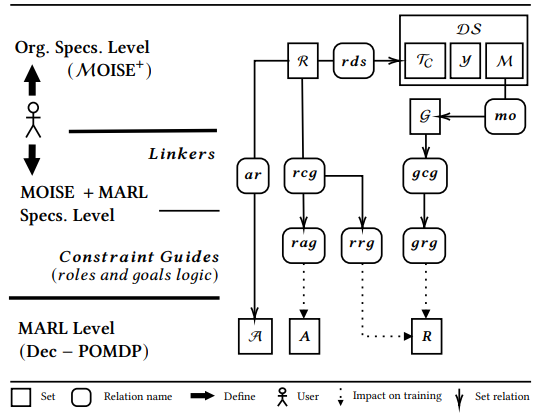
\includegraphics[width=0.6\linewidth]{figures/mm_simple_representation.png}
    \end{figure}
\end{frame}
    
\begin{frame}{Annexes}{Aperçu de PRAHOM}
    \begin{figure}
        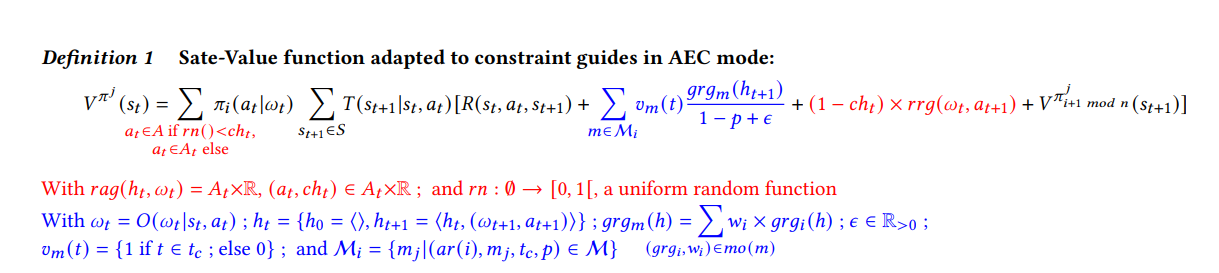
\includegraphics[width=\linewidth]{figures/modified_state_value_function.png}
    \end{figure}
\end{frame}
    
\begin{frame}[allowframebreaks]{Annexes}{Approche AOMEA : Fondement théorique}
    \textbf{Contraindre l'espace des politiques} pendant l'entraînement

    \begin{columns}
    
        \begin{column}{0.3\textwidth}
    
            \begin{itemize}
                \item À chaque étape, l'ensemble des actions disponibles est modifié pour correspondre aux contraintes de politiques définies par les utilisateurs ;
                \item Contraintes intégrées via : correction externe, apprentissage, modification interne des politiques.
            \end{itemize}
    
        \end{column}
    
        \begin{column}{0.8\textwidth}
            \begin{figure}
                \centering
                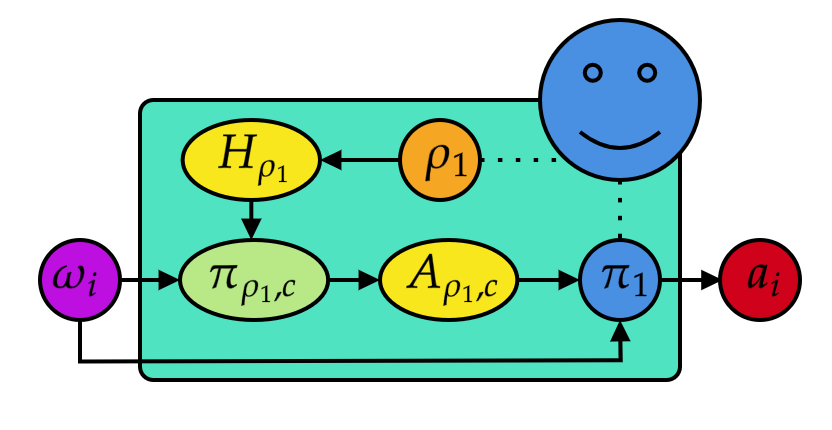
\includegraphics[width=0.7\linewidth]{figures/prahom_training_constrain.png}
                \caption*{Vue résumée de la contrainte PRAHOM}
                \label{fig:prahom_process}
            \end{figure}
        \end{column}
    
    \end{columns}
\end{frame}

\begin{frame}{Annexes}{Constrained Reinforcement Learning (Constrained-RL)}
    
    \begin{itemize}
        \item Apprendre une politique optimisant la récompense tout en respectant des \textbf{contraintes de sécurité} ou de \textbf{performance}.
        
        \item \textbf{Contraintes dures} : doivent toujours être respectées (Shielding).
        \item \textbf{Contraintes douces} : respectées en moyenne ou sous forme de pénalités.
        
        \item \textbf{Méthodes :}
            \begin{itemize}
                \item \textbf{Reward Shaping} : ajout de pénalités pour violation de contraintes.
                \item \textbf{Policy Projection} : ajustement des actions pour rester dans les limites.
                \item \textbf{Dual Variables} : intégration de multiplicateurs de Lagrange pour gérer les contraintes.
            \end{itemize}
            
    \end{itemize}    
\end{frame}

\begin{frame}{Annexes}{Safe Exploration et Shielding en Reinforcement Learning}
    
    \begin{itemize}
        \item \textbf{Safe Exploration} $\rightarrow$ garantir la sécurité lors de la phase d'exploration en limitant les risques de comportements dangereux.
        \item Principalement modifier la fonction de récompense (Langragien) pour integrer contraintes mais aussi\dots
        \item \textbf{Shielding} intervenir en temps réel pour bloquer les actions susceptibles de violer ces contraintes, permettant une exploration sécurisée.
    \end{itemize}
    
    \textbf{Référence :} \\
    \textit{Akifumi Wachi, Wataru Hashimoto, Xun Shen, \& Kazumune Hashimoto (2023). Safe Exploration in Reinforcement Learning: A Generalized Formulation and Algorithms. In Thirty-seventh Conference on Neural Information Processing Systems.}

\end{frame}

\begin{frame}[allowframebreaks]{Annexes}{Approche AOMEA: Fondement théorique}

    \textbf{Inferrer des Spécifications Organisationnelles}

    \begin{columns}

        \begin{column}{0.3\textwidth}

            \begin{itemize}
                \item \textbf{Knowledge-based Organizational Specifications Identification (KOSIA)}
                \item \textbf{General Organizational Specifications Infererence (GOSIA)}
            \end{itemize}

        \end{column}

        \begin{column}{0.8\textwidth}
            \begin{figure}
                \centering
                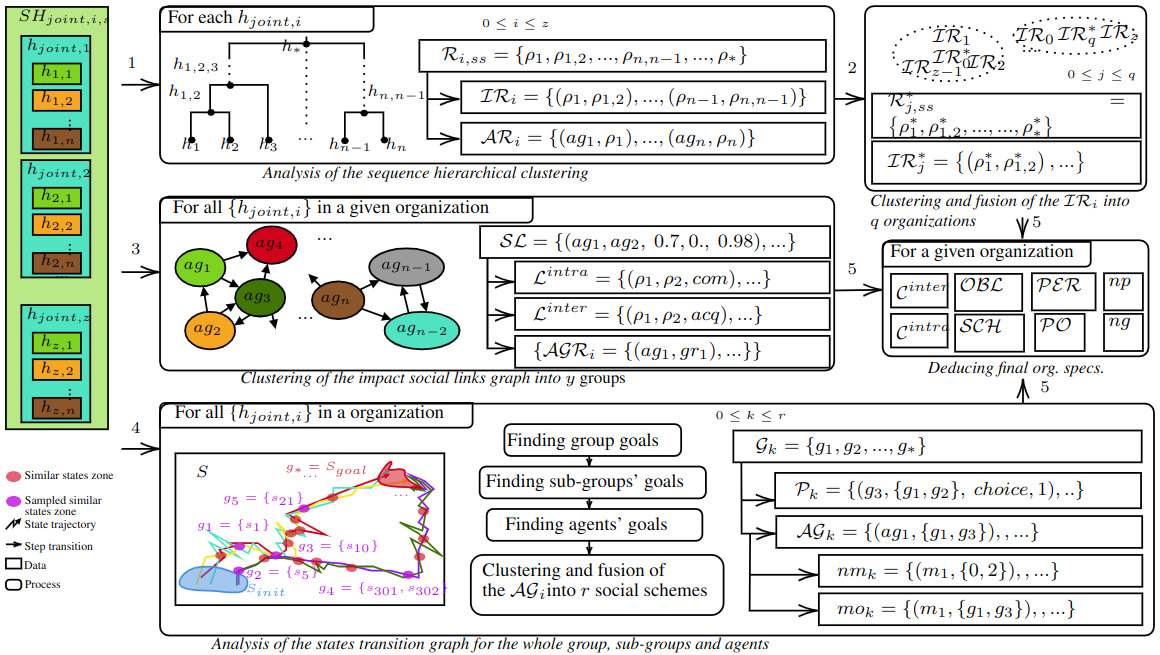
\includegraphics[width=0.95\linewidth]{figures/GOSIA_view.png}
                \caption*{A summary view of the GOSIA process}
                \label{fig:gosia_process}
            \end{figure}
        \end{column}

    \end{columns}

\end{frame}


%%%%%%%%%%%%%%%%

% Slide 2: Exemple d'utilisation
\begin{frame}[fragile]{Annexes}{Exemple d'utilisation d'Optuna}
    \begin{itemize}
        \item \textbf{Optuna} est une bibliothèque open-source pour l'optimisation des hyperparamètres (HPO), utile en apprentissage automatique.
        \item Exemples d'hyper-paramètre : taux d'apprentissage, fonction activation, nb couche, taille couches, seuil de ressemblance pour Hierarchical Clustering\dots
        \item \textbf{Étapes pour utiliser Optuna :}
        \begin{itemize}
            \item \texttt{1.} Définir une fonction d'objectif.
            \item \texttt{2.} Lancer une étude avec Optuna.
            \item \texttt{3.} Utiliser le meilleur résultat pour entraîner le modèle.
        \end{itemize}
    \end{itemize}

    \begin{lstlisting}[language=Python, basicstyle=\small\ttfamily, frame=single, caption=Exemple d'Optuna en Python]
import optuna

def objective(trial):
    x = trial.suggest_float("x", -10, 10)
    return (x - 2) ** 2 # Mock : fonction "etat-valeur"

study = optuna.create_study(direction="minimize")
study.optimize(objective, n_trials=100)

print(study.best_params)  # Affiche les meilleurs parametres
    \end{lstlisting}
\end{frame}


\begin{frame}{Annexes}{Aperçu PettingZoo}
    \begin{itemize}
        \item Bibliothèque Python pour environnements multi-agents.
        \item Simplifier l'entraînement et l'évaluation des agents dans divers environnements.
        \item \textbf{Caractéristiques principales} :
        \begin{itemize}
            \item Supporte plusieurs types d'environnements multi-agents (tour par tour, simultané, etc.).
            \item Intégration facile avec des frameworks de reinforcement learning comme RLlib.
            \item Compatible avec les API de Gym, permettant une utilisation intuitive.
        \end{itemize}
        \item \textbf{Exemples d'environnements inclus} :
        \begin{itemize}
            \item Jeux : \textit{TicTacToe}, \textit{ConnectFour}.
            \item Scénarios de collaboration et de compétition : \textit{Pistonball}, \textit{Prisoner's Dilemma}.
            \item Intégration avec la suite d'environnements Atari pour le multi-agent.
        \end{itemize}
    \end{itemize}
\end{frame}

\begin{frame}[fragile]{Annexes}{Exemple utilisation de PettingZoo}
    \begin{itemize}
        \item Exemple : Création et interaction avec un environnement.
        \item Chargement de l'environnement, réinitialisation et étapes d'interaction pour un agent.
    \end{itemize}
    \vspace{0.3cm}
    \begin{lstlisting}[language=Python, basicstyle=\ttfamily\small]
from pettingzoo.butterfly import pistonball_v6

# Creer et reinitialiser l'environnement
env = pistonball_v6.env()
env.reset()

# Boucle principale d'interaction
for agent in env.agent_iter():
    obs, reward, done, info = env.last()
    action = env.action_space(agent).sample()  # Action aleatoire
    env.step(action)
    if done:
        env.reset()  # Reinitialiser si l'episode est termine
\end{lstlisting}
\end{frame}


\begin{frame}{Annexes}{KB-Org}
    \frametitle{Organization-based multi-agent systems: From modeling to implementation}
    
    \begin{itemize}
        \item Modélisation et mise en œuvre des SMA basés sur organisation ;
        \item Intègre les concepts d'organisation pour structurer les interactions et le comportement des agents ;
        \item Banque d'organisations disponibles prêtes à être utilisé ;
        \item Explicabilité et à la coordination.
    \end{itemize}
    
    \

    Sims, V. (2008). Automated organization design for multi-agent systems. Autonomous Agents and Multi-Agent Systems, 16(2), 151-185.

\end{frame}

\begin{frame}{Annexes}{Présentation de la bibliothèque MARLlib}

    \begin{itemize}
        \item Bibliothèque Python pour MARL
        \item Supporte plusieurs environnements MARL comme PettingZoo, StarCraft II, MPE (Multi-Agent Particle Environment), etc.
        \item Implémente divers algorithmes MARL, incluant MADDPG, MAPPO, etc.
        \item Fournit une interface pour comparaison d’algorithmes, l’entraînement et l’évaluation.
        \item Offre des configurations \textit{fine-tunés} pour de nombreux environnements
    \end{itemize}

\end{frame}

\begin{frame}[allowframebreaks]{Annexes}{Présentation de la bibliothèque MARLlib}

    \begin{itemize}
        \item \textbf{Algorithmes Basés sur les Valeurs}  
        \begin{itemize}
            \item \textbf{Multi-Agent Q-Learning} : Une extension multi-agent fondamentale de Q-learning.  
            \textit{Description} : Simple à implémenter, mais avec des difficultés de scalabilité et de non-stationnarité.
            \item \textbf{MADDPG} : Une adaptation de DDPG pour les environnements multi-agents.  
            \textit{Description} : Gère bien les espaces d'actions continues, mais requiert beaucoup de données et est complexe.
        \end{itemize}
    
        \

        \item \textbf{Algorithmes Basés sur les Politiques}  
        \begin{itemize}
            \item \textbf{REINFORCE} : Une méthode de gradient de politique basique pour l'apprentissage direct de la politique.  
            \textit{Description} : Adaptable aux environnements stochastiques mais souffre de variances élevées des gradients.
            \item \textbf{Multi-Agent PPO (MAPPO)} : Une extension de PPO conçue pour les configurations multi-agents.  
            \textit{Description} : Stabilise les mises à jour, mais nécessite un ajustement minutieux et un coût de calcul élevé.
        \end{itemize}
    
        \item \textbf{Algorithmes Hybrides}  
        \begin{itemize}
            \item \textbf{A3C (Asynchronous Advantage Actor-Critic)} : Combine l'apprentissage des politiques et des valeurs pour un équilibre exploration/exploitation.  
            \textit{Description} : Accélère l'entraînement mais nécessite une synchronisation complexe.
            \item \textbf{MAPPO} : Un hybride intégrant PPO avec un entraînement centralisé.  
            \textit{Description} : Efficace pour les tâches coopératives, mais difficile dans les environnements compétitifs et exigeant en ressources.
        \end{itemize}
    
        \item \textbf{Algorithmes Théoriques et Coopératifs Basés sur le Jeu}  
        \begin{itemize}
            \item \textbf{Independent Q-Learning (IQL)} : Une version indépendante de Q-learning pour chaque agent.  
            \textit{Description} : Simple à implémenter mais avec de sérieux problèmes de non-stationnarité en multi-agent.
            \item \textbf{COMA (Counterfactual Multi-Agent Policy Gradients)} : Utilise des baselines contrefactuelles pour évaluer les contributions des agents.  
            \textit{Description} : Réduit la variance et améliore la coopération, mais demande des calculs lourds.
        \end{itemize}
    
        \item \textbf{Entraînement Centralisé avec Exécution Décentralisée}  
        \begin{itemize}
            \item \textbf{QMIX} : Décompose les valeurs Q pour améliorer la coordination multi-agent.  
            \textit{Description} : Équilibre l'entraînement centralisé et l'action décentralisée, mais moins efficace en environnements très compétitifs.
            \item \textbf{VDN (Value Decomposition Networks)} : Simplifie la coordination multi-agent avec la décomposition des valeurs.  
            \textit{Description} : Efficace mais limité dans la gestion d'interactions complexes.
        \end{itemize}
    \end{itemize}
    

\end{frame}


\end{document}
